\chapter{Introduction}
Since the first vaccine research, by Edward Jenner on smallpox, it has been clear that the human immune system is adaptable and able to protect its host from serious infections.
During the 20th century an impressive amount of basic research effort resulted in the deep understanding we have about immunology today.
Many discoveries in immunology later turned out to be directly applicable in medicine as vaccines, anti-inflammatory agents, cancer treatments etc.
Especially the area of adaptive immunity has been extensively studied due to its fascinating abilities to protect humans from bacterial and viral infection.

B and T cells and their receptors (BCRs and TCRs respectively) play a central role in the adaptive immune system which have classically been studied by low throughput techniques like microscopy, ELISA and PCR.
However, the most important part of these cells are their receptors and the binding abilities of these, which are purely sequence dependent.
After this was recognized the first sequencing studies were slowly undertaken but with no where near enough sequences to give detailed insights about BCR and TCR function.
It was first recently, around 2008, that it got possible with high-throughput pyrosequencing (Roche 454) to sequence thousands of BCRs and TCRs \cite{campbell2008subclonal}, \cite{boyd2008high}.
Since then high throughput sequencing (HTS) is becoming a standard lab technique and sequencing BCR/TCR repertoires (Rep-Seq) is now done by many academic groups as well as commercially by several companies.

Despite the initial enthusiasm around Rep-Seq, the dust has settled, revealing a slightly disappointing reality.
Slightly disappointing because Rep-Seq is, for various reasons, not answering as many scientific questions as it was initially hoped.
There has been a number of studies showing just how vast and diverse the immune receptor repertoire is \cite{zhang20173d}, \cite{elhanati2015inferring} and how there is a repertoire bias across different individuals \cite{dewitt2016public}, \cite{vander2017dysregulation}, but because BCR sequences themselves does not provide information about their function, interpretation of these Rep-Seq results are difficult and too often ends up being a hunt for significant case vs.\ control changes with little meaningful interpretation.
For example there might be a significant change in the use of certain germline genes, under circumstances of an autoimmune disease, but is this caused by the self reactive auto-antibodies or is the change in gene usage just a side effect of the disease's influence on the repertoire?
A question like this is difficult to answer without extra information about the function of the antibody present in the sample and therefore conclusions drawn from changes in germline gene usage lack causality.
However Rep-Seq is still in its infancy and indeed is starting to find a niche of applications e.g.\ lineage tracing for vaccine response \cite{Doria-Rose2014-vi}, \cite{Wu2011-yj} and in antibody discovery applications \cite{reddy2010monoclonal}.

Missing functional information about the sequences from Rep-Seq data is what makes it difficult to interpret because there is no known truth to use as a reference.
E.g.\ it cannot be known exactly which B cells are sharing the same common ancestor cell (clonal relationship), it can only be inferred from sequence similarity and epitope binding specificity.
Most often epitope binding specificity it not available for each cell so clonal relationship is inferred solely based on sequence similarity with no test to validate this assumptions.
In such cases when sequence information is rich, but functional and relational information is sparse, or non-existing, the importance of simulation studies cannot be understated.
Simulating the missing information is often the only way to validate Rep-Seq analysis tools and therefore there is a real need for setting up simulation protocols mimicking real Rep-Seq data.

In this work I will present tools and methods for simulating the phylogeny of B cells evolving in a germinal center (GC) reaction, and then apply the simulated sequences to validate phylogenetic methods.
In order to achieve this a new method for integrating affinity selection into tree simulation is derived, along with a new metric for assessing the correctness of an ancestral sequence reconstruction.




\chapter{Practical and theoretical considerations}
Integrating HTS data into immunological research is a challenge that requires insight in many aspects, ranging from basic cellular pathways of the immune system to statistical modeling and advanced data analysis.
Even when the objective is to build a purely statistical model there are many benefits to be drawn from having a solid knowledge about the pathways governing the immune system, and likewise it will avoid many pitfalls to have practical experience with sequencing data, read processing, quality control etc.

In this chapter I will describe the theoretical fundamentals that makes the foundation for the chapters to follow, mixed with some of the practical considerations that are important but somewhat implicit knowledge in the field.



\section{Adaptive immunity}
The function of the immune system is to protect its host against invading pathogens.
To carry out this job the effector cells of the immune system have been equipped with a license to kill, and not only to kill pathogen, but also to kill its own host cells.
With this potential harmful weapon the immune system needs to be tightly regulated to balance between fighting off pathogens while doing least possible harm on the host.

At the lowest level of classification the immune system is split up into innate and adaptive immunity.
As the name suggested the innate immunity is hard coded in the genome and cannot change during the course of an infection.
The opposite is true for the adaptive immunity, this is not hard coded in the genome and is undergoing development throughout the course of an infection.
Innate immunity is the oldest of the defense mechanisms, adaptive immunity came along later giving a large selection advantage to the host, but always on the terms of the innate immune system.
The innate immune system is broadly defined as both the physical barriers, like skin, mucous, stomach acid etc. but also covers cells like macrophages, dendritic cells and the proteins of the complement system.
The adaptive immune system includes less elements and is defined as the cells of the B and T cell lineages.
There is a tight interaction between the two systems and events in the innate system can cause activation of elements in the adaptive and vice versa, see figure \ref{fig:innate_and_adaptive}.

To get a more complete picture of the processes involved lets walk through an example of a simple bacterial infection cause by a skin tear.
At first bacteria enters the blood stream where they start proliferating, but some are also getting engulfed by macrophages.
A macrophage will process the engulfed bacteria in small intracellular membrane vesicles (called lysosomes), first by killing and thereafter by chopping up the lysosome content.
Among the content of the lysosomes will be short bacterial peptides that was previously part of full-sized bacterial proteins, and these peptides are then loaded into special surface receptors called the major histocompatibility complex class II (MHCII) and presented on the surface of macrophages circulating through the blood stream.
At the same time a large number of T cell with different TCRs are monitoring the blood and some will carry a TCR that binds specifically to an MHCII presenting a bacterial peptide on the surface of a macrophage.
As a result of binding the macrophage activates the T cell to undergo proliferation and a burst of T cells with identical TCRs will emerge (clonal burst).
At the same time a large number of B cells with different BCRs are monitoring the blood stream binding a variety of different proteins, and whatever these B cells bind to their BCRs are getting transported into the cell, chopped up and presented in MHCII is a similar fashion as the macrophages (this is a highly idealized description of antigen sequestering and presentation, for a detailed mechanistic review see \cite{batista2009and}).
Some of these B cells will bind proteins from the immunizing pathogen and present peptides from these protein in MHCII on its cell surface.
Now some of these MHCII:peptide complexes are identical to the ones presented on the macrophages, and the recently clonally expanded T cells will bind them and activate the B cells to undergo a number of maturation steps, discussed in details later in this section.
The result is secretion of large quantities of antibodies (a secreted form of a BCR) that binds to the surface proteins of the bacteria and thereby signalling the complement system and other immune cells to clear the infection.
Sometimes the unspecific engulfing of extracellular fluids by macrophages will not be efficient enough to clear a bacterial infection, but once flagged with antibodies, clearance can be mediated by the complement system and occur rapidly.

\begin{figure}
    \centering
    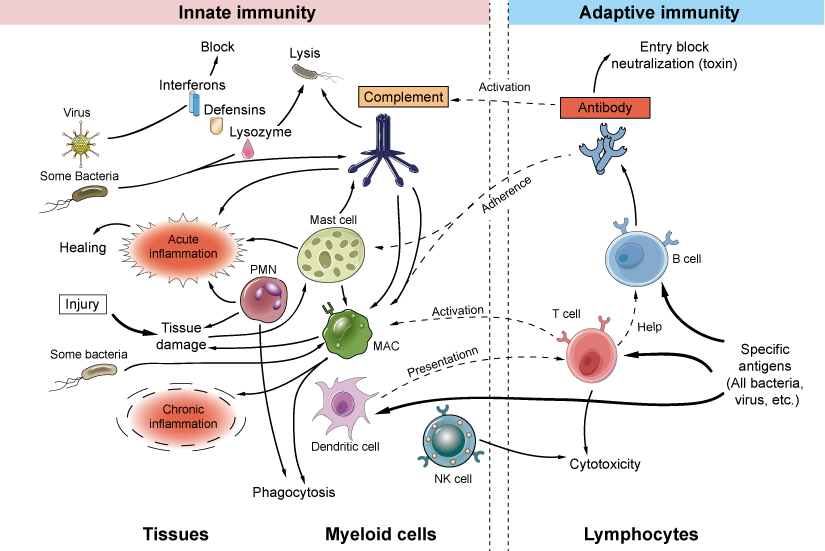
\includegraphics[width=0.9\textwidth]{figures/innate_and_adaptive.png}
    \caption{
        \label{fig:innate_and_adaptive}
        Connection between the innate and adaptive immune system.
        Macrophage (MAC), Polymorphonuclear leucocyte (PMN), Natural killer (NK).
        From \url{http://www.creative-diagnostics.com/innate-and-adaptive-immunity.htm}.
    }
\end{figure}


In summary, we can think of adaptive immunity, in a highly idealized and simplistic way, as going through the following steps:
\begin{itemize}
  \item An antigen presenting cell (e.g.\ a macrophage or dendritic cell) engulfs a foreign protein and presents a its peptide in MHCII.
  \item A T cell clone with TCRs binding this MHCII:peptide complex gets clonally expanded.
  \item A B cell clone binds the same foreign protein, engulfs it and presents its peptides in MHCII.
  \item The clonally expanded T cells bind these MHCII:peptide complexes, inducing B cell proliferation and the production of antibodies.
\end{itemize}
Each item on the list has many details omitted for the sake of simplicity, but one thing missing and worth to highlight is the concept of memory.
The list ends with clearance of the infection through secretion of antibodies binding the pathogen, but this process is slow and very energy consuming, so keeping a memory of the pathogen is an important mechanism to mount rapid response towards repeated infections.
Immune memory is build by immortalizing T and B cells involved in the adaptive immunity reaction of the first encounter with a pathogen, then whenever the same pathogen is encountered again, memory cells will quickly be able to start attacking the invasion.







\subsection{B cell receptors}
The adaptivity of adaptive immunity lies in the diversity of BCRs and TCRs.
Like so many receptors involved in the immune system both BCRs and TCRs are built up by protein domains from the immunoglobulin superfamily.
But unlike other receptors in the immune system they are not encoded by a single gene but by several genes stochastically recombined from multiple loci.
Mechanisms of generation of BCRs and TCRs are so overlapping that it will be sufficient in the following section to only describe the mechanism of generating BCRs.

Antibodies are the secreted form of a BCRs having with the same structure except for the missing membrane anchor.
A BCR is a tetrameric protein of two pairs of identical chains referred to as the heavy and light chains because one is longer than the other, see a) in figure \ref{fig:BCR_structure2}.
The heavy/light chain pairs are linked together covalently by disulfide bonds, likewise are the two heavy chains from each pair, making a BCR a very stable structure.
Both chains starts with a variable region that defines the antigen binding ability of an antibody, and ends with a non-variable constant region (CH1-3/CL).
The number of different variable regions found in a sample of naive (non antigen experienced) human B cells reveal that there are orders of magnitude more different BCRs than single genes on the genome.
Instead of being gene encoded this diversity is introduced by recombining several pieces of DNA from different loci into a full-sized variable region, see b) in figure \ref{fig:BCR_structure2}.
These segments are called the germline genes and for heavy chain sequences there are three groups, the variable (V), the diversifying (D) and the joining (J).
These V, D and J germline gene groups have multiple variants existing in sequential order on the chromosome, and during a stochastic process called VDJ recombination, one of the genes from each germline gene group is physically spliced together into a full-size variable region VDJ gene.
Coupled to a constant region gene further downstream this is being transcribed and translated into one of the heavy/light chains of a BCR protein.

\begin{figure}
    \centering
    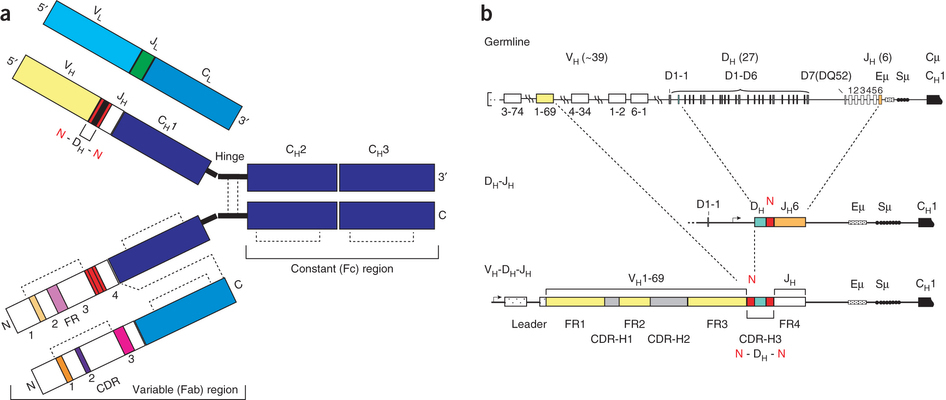
\includegraphics[width=1\textwidth]{figures/ab_structure.jpg}
    \caption{
        \label{fig:BCR_structure2}
        Antibody structure and germline organization on the genome.
        From \cite{georgiou2014promise}.
    }
\end{figure}


While VDJ recombination is not a completely random process \cite{li2012recombinatorial}, it is the basis of all the variability in the variable region in a BCR sequence.
But the combinatorics of all the germline genes are only modest, $\approx 39\times27\times6=6318$ different VDJ combinations times two (due to humans being diploid organisms), vastly less than what is observed in experimental studies.
The rest of the observed diversity comes from another stochastic process involving trimming and inserting new nucleotides at those DNA ends that are joined together, see figure \ref{fig:VDJ_recomb}.
The extra nucleotides added in the junction between V-D and D-J are called N/P nucleotides and the length of these indels can vary from zero to tens of nucleotides.
Although the observed distribution of junctions lengths is not uniformly random, and there is a bias in the inserted nucleotides \cite{murugan2012statistical}, \cite{elhanati2015inferring}, N/P nucleotides adds orders of magnitude more diversity to the combinatorics of gene recombination.
Furthermore all the junctional diversity is contained in the third complementarity defining region (CDR), as opposed to the framework region (FR), see figure \ref{fig:VDJ_recomb}.
As the name suggests the CDR is the structural region that binds the antigen, and to enable binding of a wide range of structures this region must be highly diverse.
Based on a combination of gene recombination and junction diversity and weighted by their distributional biases, Elhanati et al.\ estimated that the naive repertoire is $10^{16} - 10^{18}$ productive sequences \cite{elhanati2015inferring}.
The sequences resulting directly from VDJ recombination and N/P bases are referred to as naive sequences to reflect that these are in a stage before antigen experience and germinal center maturation explained later.
All this diversification occurs within all individuals in the B cell generation in the bone marrow, however with the subtle difference that VDJ genes can differ between individuals.
The different VDJ genes are called alleles and have the potential of expanding the binding breadth of the population wide BCR repertoire even further.

\begin{figure}
    \centering
    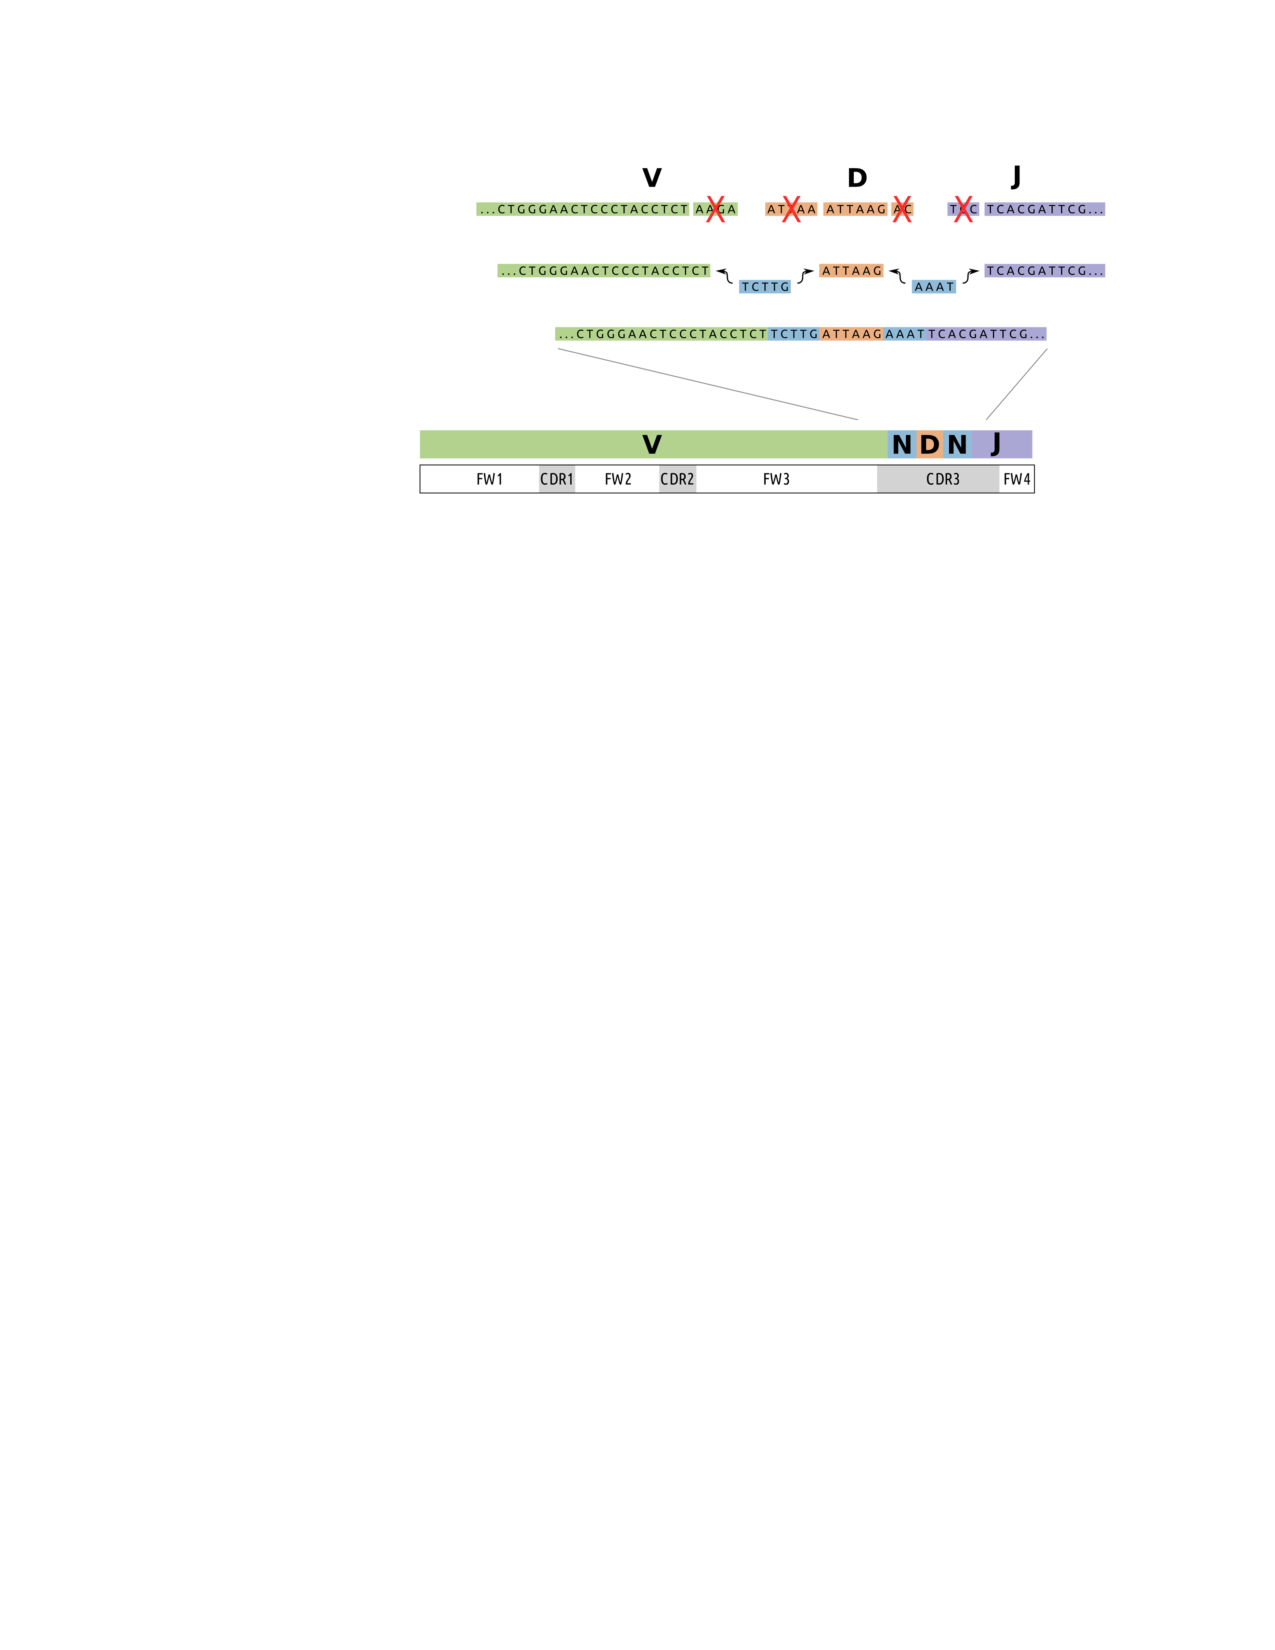
\includegraphics[width=0.7\textwidth]{figures/VDJ_recomb.pdf}
    \caption{
        \label{fig:VDJ_recomb}
        VDJ recombination and introduction of junctional diversity by exonuclease activity and N/P nucleotides added to the joining ends.
        From \cite{ralph2016consistency}.
    }
\end{figure}


While the above description covers the concepts of BCR diversification in general it was applied specifically to an example of a heavy chain variable sequence.
The light chain variable sequence is generated by similar recombination, but light chains do not have the D germline gene and therefore only performs a VJ recombination with substantially less junctional diversity.
Light chain germline genes are present in two non-identical copies named kappa and lambda residing on different chromosomes.
The light chain sequence will only be expressed from one of these, the choice of which is determined by a selection process in the bone marrow excluding self-antigen binding BCRs.
Pairing of a heavy and light chain sequence yields an even larger possible naive repertoire, and with a production rate of at least $10^7$ naive B cells per day \cite{murphy2008immunobiology}, it is not surprising that the adaptive immune system can recognize nearly all foreign antigens.
With such a broad range of antigen binding there will naturally be many BCRs binding endogenous proteins (self-antigens).
This is not desirable because it would lead to immune attach against host cells, known as autoimmunity, and therefore the adaptive immune system has a strict selection process in the bone marrow to destroy B cells with non-functional or self-antigen binding BCRs.
A similar process is happening for T cells in the thymus.




\subsubsection{Germline nomenclature}
The standard nomenclature for BCR genes used throughout this work is defined by the IMGT ontology summarized in figure \ref{fig:IMGT_classification} and described by Lefranc \cite{lefranc2001nomenclature}.
The first part of the gene name is always "IG" and followed by a locus identifier that can be either H (for heavy chain), K or L (for kappa or lambda light chain).
The next letter represents the gene group which can be V, D or J for the variable region, and for the constant region the different isotypes e.g.\ A, E, G1, G2 etc.

\begin{figure}[ht]
    \centering
    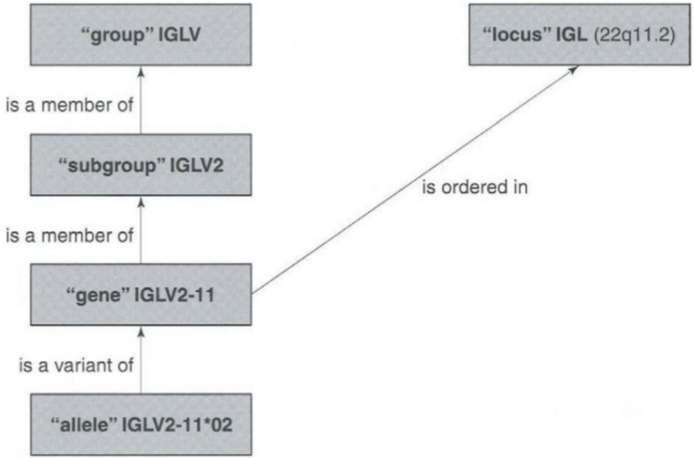
\includegraphics[width=0.6\textwidth]{figures/IMGT_classification.png}
    \caption{
        \label{fig:IMGT_classification}
        IMGT germline gene ontology.
        From \cite{giudicelli1999ontology}.
    }
\end{figure}


For the variable region gene group additional layers of nomenclature are needed since there are many different V, D and J genes under each group.
The first layer is the subgroup level which is defined as a cluster of genes sharing at least 75\% nucleotide similarity.
There are 7 of these subgroups in IMGT and presumably they each derive from distinct gene duplication events, an interpretation supported by the distances separating subgroup genes on their inferred phylogeny, see figure \ref{fig:IGHV_tree}.
However the subgroup level is \textit{not} defined phylogenetically, even though it might coincide with a phylogenetic interpretation.

\begin{figure}
    \centering
    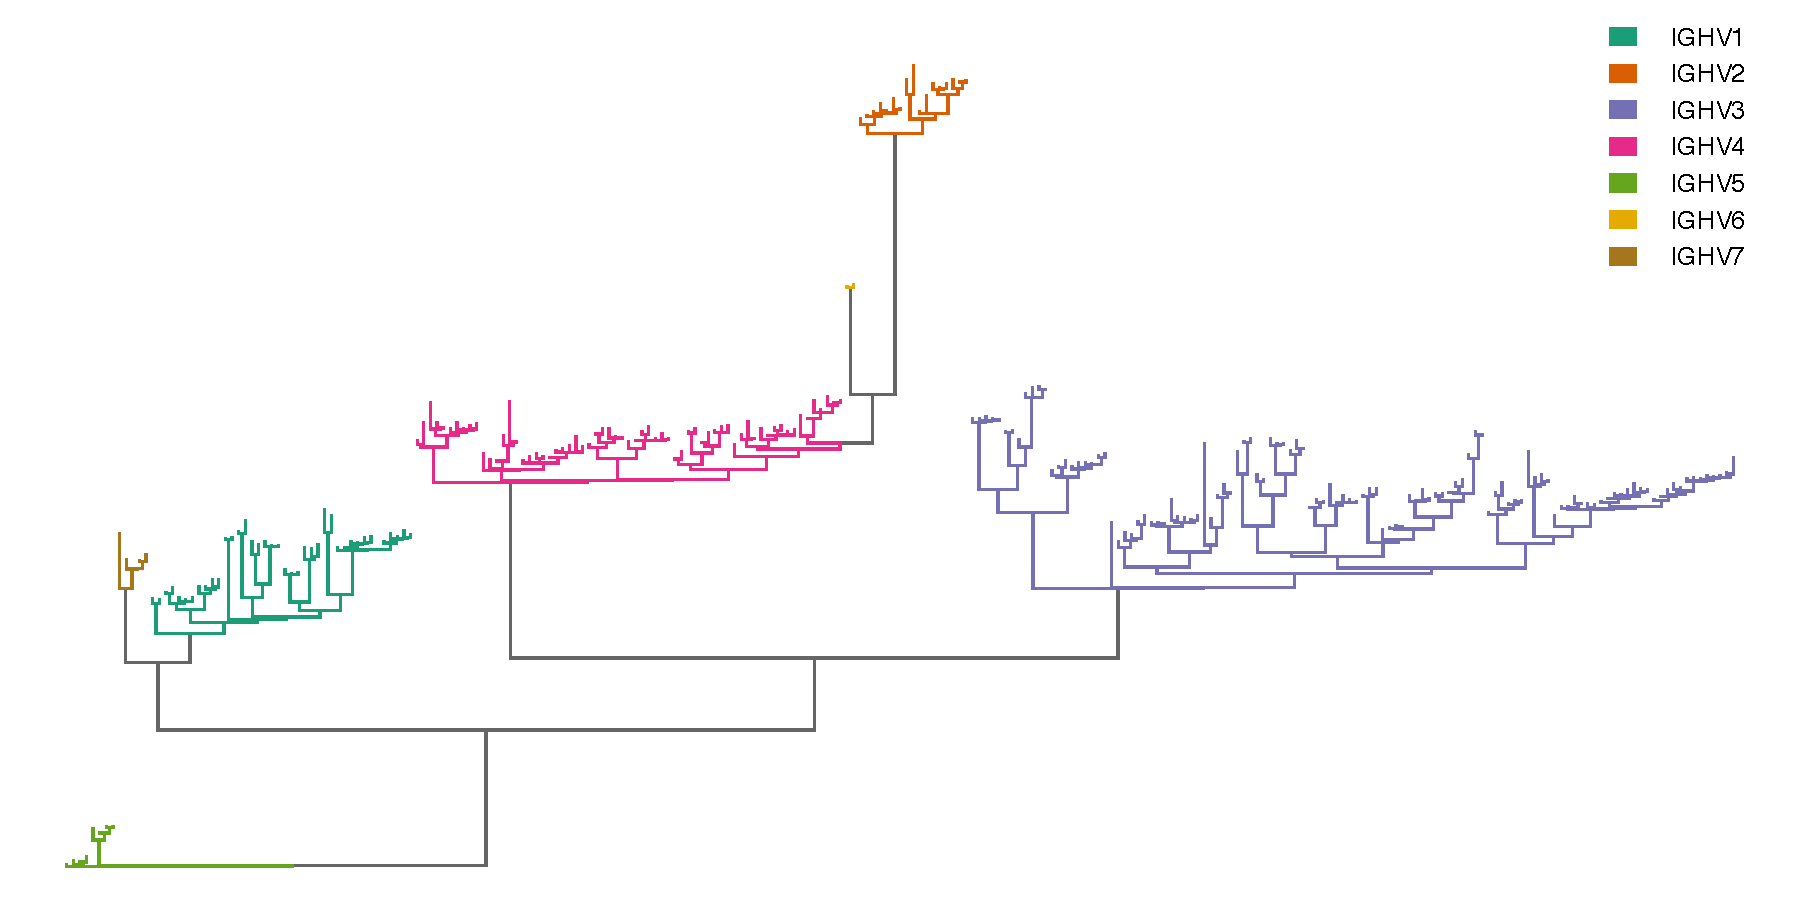
\includegraphics[width=1\textwidth]{figures/tree_right_side_up.pdf}
    \caption{
        \label{fig:IGHV_tree}
        Tree of germline V genes.
        All IGHV alleles were downloaded from IMGT, pseudo genes were removed and a multiple sequence alignment generated with BAli-Phy \cite{suchard2006bali} and MAFFT \cite{katoh2013mafft}.
        BAli-Phy was also used in tree inference, given a fixed topology within each IGHV subgroup determined by RAxML \cite{stamatakis2008rapid}.
        Figure credit: Andy Magee.
    }
\end{figure}


Each subgroup has a number of genes that are defined by their chromosomal position (locus) and present in all individuals in a species.
Each gene is encoded by a single sequence, the allele, that can vary between individuals and will by present in two copies, one on each chromosome.
A gene can have many different observed alleles in a population, and while these allelic differences between individuals are usually just single nucleotide polymorphism, indels do occur causing some alleles of the same gene to have different length.

The rules described above is the intended IMGT nomenclature, however it turns out that gene duplications/deletions are commonly observed at the immunoglobuline locus in both humans \cite{scheepers2015ability} and other animals \cite{collins2015mouse}, \cite{corcoran2016production}, and hence it is not certain that all individuals will have the same number of genes on the same chromosomal locations.
This presents a large problem for germline annotation and mutation frequency estimation and as of now this is still an unresolved problem.
However, for a majority of the human data, the germline gene set is comprehensive enough that no major errors are expected, and in this case IMGT nomenclature can be used reliably.
Nonetheless, it is worth to keep in mind that gene duplications/deletions can be a problem, especially with data derived from non-European individuals \cite{scheepers2015ability}.







\subsubsection{Antibody numbering}
For both B and T cell receptors the huge diversity of the variable region is obvious on the sequence level, but much less so on the protein structural level.
Actually even the variable region of a highly mutated BCR is strictly following the structural constraints of the beta-sheet sandwich structure of the immunoglobulin domain.
Structural conservation enables consistent mapping from the amino acid sequence onto a protein structure.
A mapping like this was first proposed as a numbering scheme where the immunoglobulin structural components are numbered and these numbers are mapped back to the linear amino acid sequence.
First attempt on this was described by Kabat \cite{national1983sequences} and based on invariant residues and rule based matching (these rules are tabulated by Dr. Andrew Martins \url{http://www.bioinf.org.uk/abs/}).
Unfortunately this scheme not good at handling insertion in the flexible CDR regions, e.g.\ CDR1 insertions and/or very long CDR3 \cite{martin2010protein}.
Years later came another numbering scheme named after the first author of Clothia et al.\ \cite{chothia1987canonical}.
The Clothia scheme was set out to correct the wrong mapping of CDR1 insertions and thereby achieve structurally consistent mapping, but later this has been updated to also accommodate structural consistent mapping of framework indels.

In 2003 the IMGT numbering was proposed to unify numbering of BCRs and TCRs \cite{lefranc2003imgt}.
Similar to the IMGT scheme another scheme, called AHo, was made unifying numbering of BCRs and TCRs \cite{honegger2001yet}.
Like Clothia, AHo numbering is structurally consistent, but unlike any other scheme it has a fixed standard length of 149 positions with enough space for even very long CDR3 sequences.
Only in rare cases of germline indels, or an extremely long junctions, the scheme has to use insertion codes, which are otherwise standard use in all other numbering schemes.
This fixed length sequence numbering make analysis much more convenient and results easy to interpret e.g.\ all BCR sequences can be encoded by a vector of length 149 and a given position in this vector always correspond to the same position on the protein structure regardless of the sequence.
Therefore whenever BCR numbering is used throughout with work AHo numbering will be used if nothing else stated.
The software ANARCI is used to annotate BCR sequences with AHo numbers \cite{dunbar2016anarci}, (\url{http://opig.stats.ox.ac.uk/webapps/sabdab-sabpred/ANARCI.php}).

With a numbered BCR sequence also comes the rather arbitrary decision of how to define the framework and complementary defining regions (CDRs/FRs).
Clearly FRs are suppose to be more conserved and less structurally flexible while CDRs are suppose to be flexible and highly variable, but putting a boundary between them is a context dependent problem, that depends on the problem at hand.
In this work FRs are considered to be the most structurally conserved beta-sheets in the immunoglobulin domain, and CDRs are considered to be the structurally flexible loops connecting these beta-sheets.
This definition is recapitulated in the CDR centric numbers tabulated by Andreas Pl{\"u}ckthun (\url{https://www.bioc.uzh.ch/plueckthun/antibody/Numbering/}).
The FR1-4 ranges are: \texttt{1-27, 41-57, 78-108, 138-149} and the CDR1-3 ranges are: \texttt{28-40, 58-77, 109-137}.






\subsection{Biology of the germinal center reaction}
It was discovered by Eisen and Siskind already in 1964 \cite{eisen1964variations} that antibody affinity was increasing during the course of an immune reaction.
The phenomenon is known as affinity maturation and by employing single cell techniques for staining, sorting and sequencing it has now been revealed that maturation is driven by a Darwinian selection process spatially confined into small nodules called germinal centers (GCs) residing in lymph nodes.
Affinity maturation typically starts in the GCs 6 days after immunization and ends 4 weeks later when the GCs are dissolved and GC B cells die from apoptosis \cite{victora2012germinal}.
Before dissolving, a GC will export plasma cells, that secretes large quantities of high affinity antibodies, and memory B cells that will work as a permanent memory to be quickly re-initiated upon repeated antigen exposure.
%after the death of plasma cells.

\begin{figure}[!ht]
    \centering
    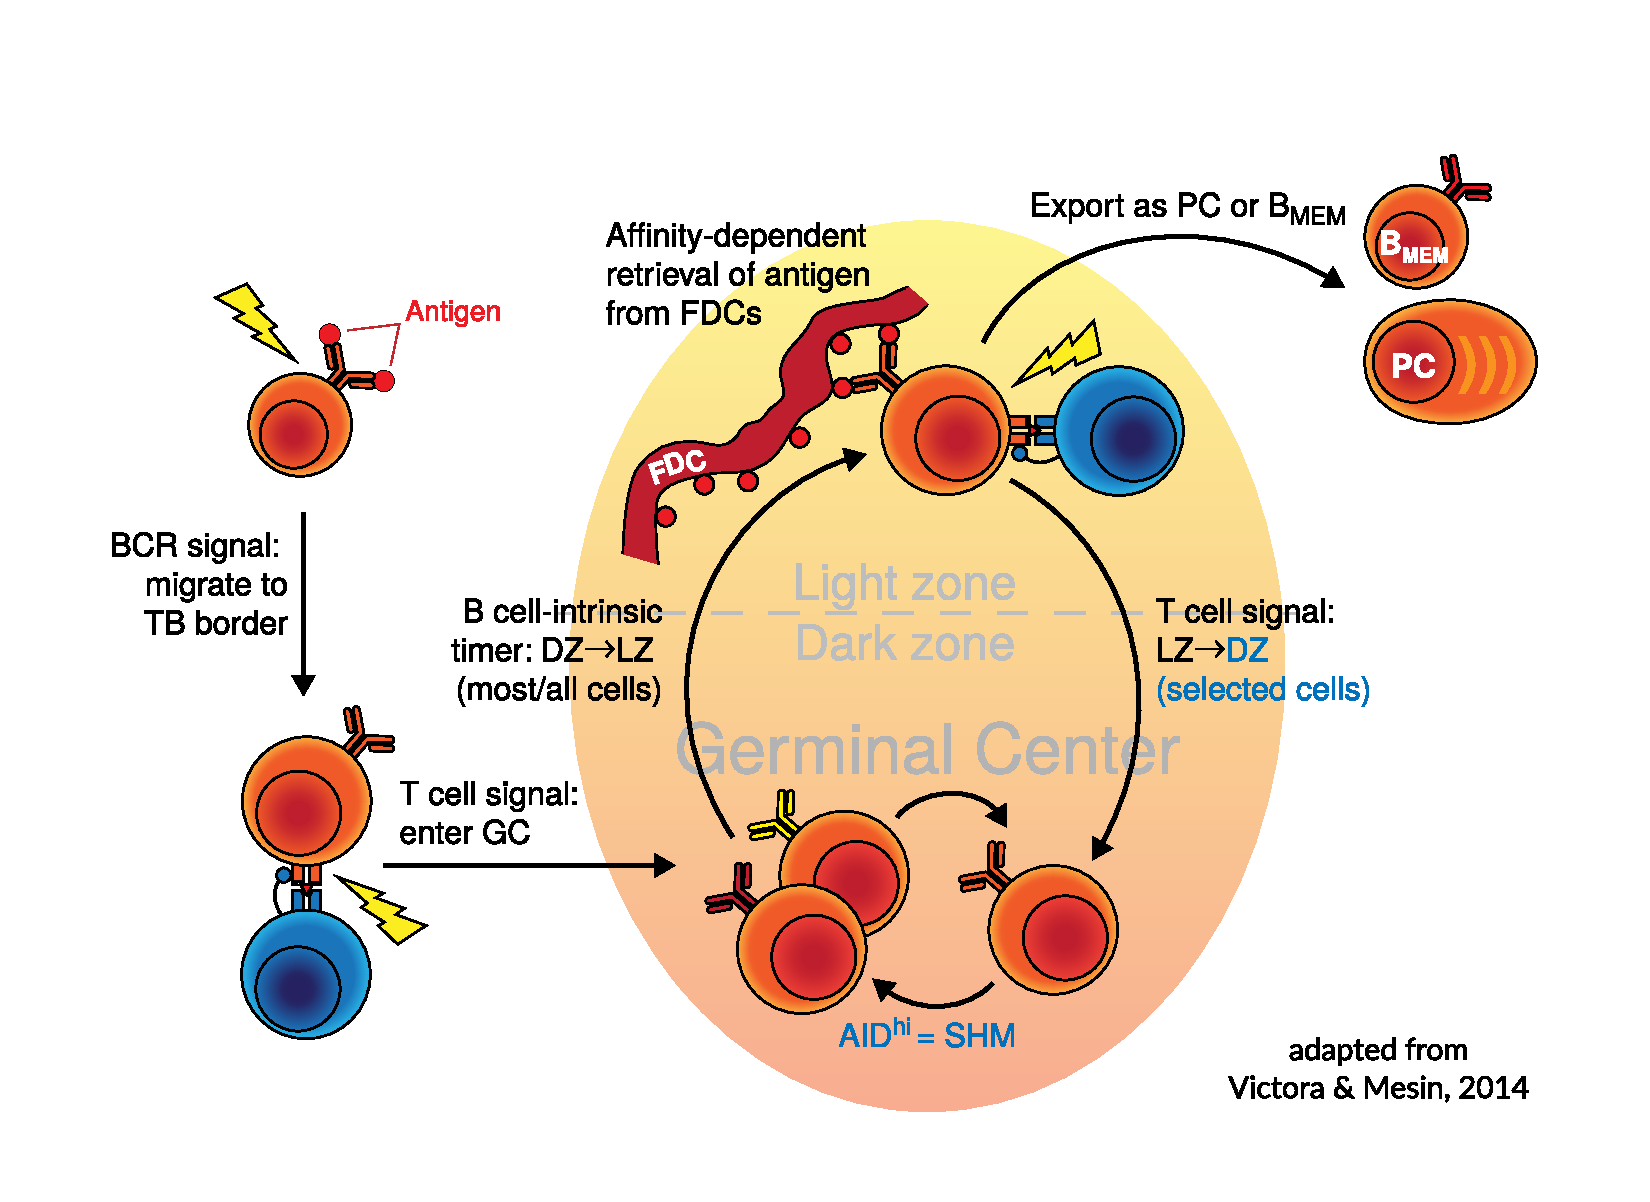
\includegraphics[width=0.6\textwidth]{figures/GC_reaction.pdf}
    \caption{
        \label{fig:GC_reaction}
        Dynamics of the GC reaction, adapted from \cite{victora2014clonal}.
        Follicular dendritic (FDZ) cell in red, T follicular helper (Tfh) cells in blue and B cells in orange.
    }
\end{figure}


Taking a step back, the formation of a GC starts with an immune reaction against an antigen.
Two things are required in the initial phase, a) T cells with a TCR specific for an MHCII-peptide, with the peptide from the antigen and b) B cells with a BCR that can bind the whole antigen, engulf it and present its peptides in MHCII for the T cells to bind, see figure \ref{fig:GC_reaction}.
When these two requirements are fulfilled GC foci will start to form in the lymph nodes.
A GC is a micro-environment containing follicular dendritic cells (FDCs), T follicular helper (Tfh) cells and of course B cells.
The FDCs are antigen storage cells, they engulf large amounts of whole immunogenic proteins and slowly presents them intactly on the cell surface where they can be extracted by B cells.
The B cells undergo a mutation/selection process with two elements a) T cell help and selection and followed by b) mutation and proliferation.
The two elements are spatially separated in the GC and defined as the light zone (LZ) and the dark zone (DZ), called so because the dark zone is more densely populated with cells and appears darker when viewed under the microscope.
In the LZ B cells are attracted to the large surface of the FDC membrane through secretion of the chemokine CXCL13, some B cells will have BCR affinities strong enough that they are able to release antigen from the FDC membrane \cite{suzuki2009visualizing}.
Bound and released antigen will be engulfed, processed and presented in MHCII molecules for the Tfh cells to bind.
The more antigen a B cells is sequestering, the more peptide is presented and the more Tfh binding will occur.
If sufficient Tfh binding is achieved the B cell is signaled to migrate to the DZ by following another chemokine called CXCL12.
In the DZ it proliferates while expressing high levels of the somatic hypermutation (SHM) inducing enzyme activation-induced cytidine deaminase (AID).
With an approximate mutation rate of $10^{-3}$ per position per cell generation ($10^{6}$ higher than the normal rate) and a cell cycle time of only 6-12 hours, a large amount of variability is introduced in the DZ cells \cite{victora2012germinal}.
Eventually the progeny cells re-enter the LZ and the SHM induced variability will undergo selection, thereby completing the cycle.
B Cells are constantly cycling between LZ and DZ by switching between high expression of chemokine receptor CXCR5 and low expression of CXCR4 to migrate towards chemokine CXCL13 in the LZ, and low expression of CXCR5 and high expression of CXCR4 to migrate towards CXCL12 in the DZ.
This process is called cyclic re-entry and it continues until the GC dissolves.
During selection there are a limited amount of Tfh cells, so this is where B cells have to compete to get the activation signal.
The more antigen a B cell can sequester relative to the others, the more likely it is to get Tfh help, migrate to the DZ and go to proliferation, as oppose to undergoing apoptosis if Tfh help is insufficient.
A fraction of the B cells in the LZ will get a special Tfh differentiation signal and these are exported outside of the GC with fate as either a plasma cell or a memory cell.

While many mechanistic details of the GC reaction is known much remains to be elucidated.
The mechanisms of selection has been difficult to study but current evidence suggests that it is solely mediated through T cell interaction \cite{victora2012germinal}, \cite{victora2014clonal}.
Indeed using Tfh interaction as a model for understanding the observations, it is possible to explain all the modes of selection.
Selection can be split into three main elements:
\begin{itemize}
  \item Affinity
  \item Stability and expression
  \item Non-self binding
\end{itemize}

To improve antigen affinity is the most obvious point for selection to occur on.
A gain in BCR affinity will enable a B cell to sequester more antigen from the FDCs and present more MHCII:peptide to the limited number of Tfh cells.
Those B cells that have many MHCII:peptide complexes are much more likely to interact sufficiently to get the signal for proliferation, meaning that higher affinity is positively selected.
An extension to this is in the case of mutations altering the stability and/or expressing of a BCR, resulting in less BCRs to be presented on the cell surface.
Lower BCR levels on the cell surface will cause less antigen sequestering from the FDCs resulting in less Tfh cell interaction and causing negative selection.
Finally a more convoluted example of Tfh cell mediated selection is the negative selection of self binding BCRs.
%It has been suggested that self antigen binding B cells will mostly present self antigen derived peptides in MHCII because of the large quantities of self antigen compared to the immunizing antigen \cite{Sabouri_2014}, \cite{Bannard_Cyster_2017}.
Self antigen binding B cells are simply clogging up MHCII molecules with self peptides leading to less T cell help, and again easily explained by a Tfh cell mediated selection process.

Despite the convincing mechanistic models it must be stressed that the GC reaction contains many, either mechanistically unknown, or purely stochastic elements.
E.g.\ even though there is an observed relationship between clonal bursts and mutational gain in affinity, this does not appear to happen consistently i.e.\ large affinity gains are observed without clonal bursting \cite{tas2016visualizing}, leading to the conclusion that either the reaction is highly stochastic, or a mechanism is unknown or unmonitored e.g.\ higher affinity but worse expression could make the net balance of selection turn negative, while it appears to be positive if only looking at affinity.

A notable case of a correction to the mechanistic understanding of the GC reaction happened recently.
In 2012 a review by Victora, based on all previous evidence, suggested that GCs are initially colonized by little as 1-3 naive B cells \cite{victora2012germinal}.
However just 4 year later the same author concluded in Tas et al.\ \cite{tas2016visualizing} that this number was largely underestimated.
Using an elegant set of experiments, they were able to visualize the colonization of GCs in multiple lymph nodes across different animals and concludes that mice GCs are consistently being colonized by 50-200 naive B cells.
Before the Tas et al.\ paper in 2016 it had been a good approximation to assume that GCs were being founded by just a single cell, and that this monoclonality would be upheld throughout the entire GC reaction.
The GC identify was therefore a convenient definition of what a B cell clone is, but this view has to be redefined with the findings that GCs are starting out as highly polyclonal, and even ends up with a substantial fraction that keeps being polyclonal throughput the whole GC reaction.
Complicating things further, Tas et al.\ also observed that B cells with the same naive sequences was found across multiple GCs.
It would be fair not to distinguish between B cell clones with identical naive sequences, but matured in different GCs, as long as they mature against the same antigen, because then they undergo the same selection pressure.
But two distinct clones would need to be defined if two B cells with the same naive sequence were independently matured towards different antigens.
However it is a) practically very difficult to distinguish clones that have identical naive sequence and b) very unlikely that the exactly same BCR nucleotide sequence will mature towards more than a single antigen.
Therefore this impractical definition of a B cell clone is discouraged and instead, the simple definition from Ralph et al.\ \cite{ralph2016likelihood}, is used throughout this work.
In this scheme if two different BCRs are derived from an identical naive DNA sequence, they are in the same clonal family regardless of the GC context they came from.

SHM is driven by the enzyme AID that works by deaminating cytosines during DNA transcription.
DNA repair enzymes are then recruited to the deaminated cytosines where they with some probability will introduce point mutations both at the site of deamination and at neighboring sites.
Increased mutation rate during SHM is therefore the combined effects of AID and a number of DNA repair enzymes.
With a whopping $10^6$ times increase in mutation rate during SHM (from $10^{-9}$ to $10^{-3}$ mutations per bp per cell generation) there is a need to contain SHM so it does not destroy the function of the cell itself.
SHM achieves this by working preferentially close to the chromosomal location of the variable region genes \cite{Yeap_2015}, \cite{liu2008two}.
In addition SHM appears to be biased and preferentially introduce mutations in some contexts rather than others, incidentally this context is over represented in the variable chain genes.
The contextual bias of AID was initially described as hot/cold spots defined by a few specific 3-mer motifs (WRC/GYW hotspots and SYG/GRS coldspots) observed to change mutation rate significantly by preferentially recruiting AID \cite{pham2003processive}.

It can be difficult to tease apart the different biases introduced by both AID and the DNA repair enzymes, and though the majority of the observed SHM bias most likely comes from preferential AID activity \cite{Pham_2016}, it is their combined effect that is observed as SHM during affinity maturation.
Instead of a mechanistic model of SHM an empirical context model can be setup purely based on a large number of observed mutations and their nucleotide context.
Such a model has been described by Yaari et al.\ \cite{yaari2013models} and later in an improved version called S5F \cite{cui2016model}.
The S5F model is simply the complete set of 1024 5-mer DNA motifs and the relative probability of observing the middle base mutating.
Given a motif and a mutation on its middle base, the S5F model also provides the probability of the nucleotide identity of the resulting mutation.
A motif model is completely empirical and relies on the input data which is a large number of BCR sequences that have undergone SHM.
A survival model \cite{cox1992regression} is a good way to describe the observed data, with the event rate Theta, being proportional to the logarithm of the mutation rate of the motif (unpublished data from David Shaw and Jean Feng), see figure \ref{fig:SAMM_plot}.
Fitting the model is non-trivial, because neighboring motifs share the same context and in the case of an observed event in one motif this changed the context, and thereby Theta, in the other motifs.

\begin{figure}[!ht]
    \centering
    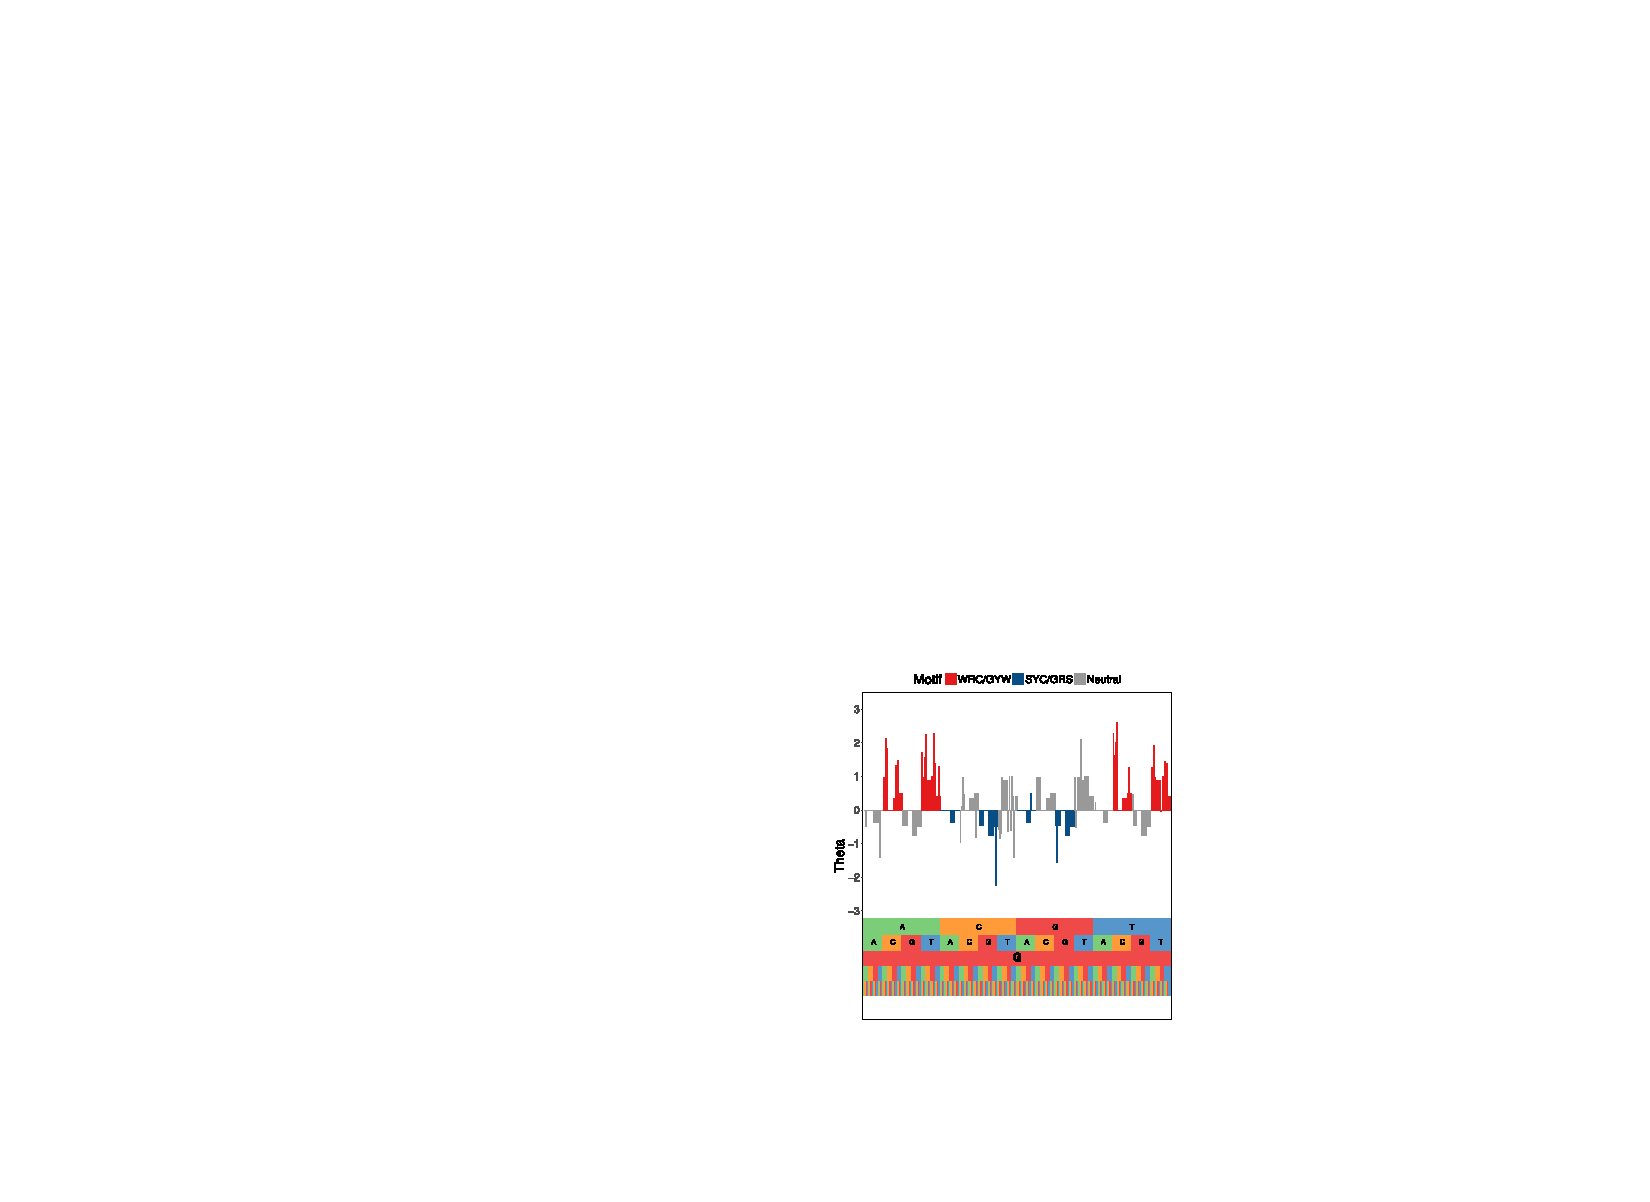
\includegraphics[width=0.45\textwidth]{figures/SAMM_plot.pdf}
    \caption{
        \label{fig:SAMM_plot}
        Plot of a 5-mer SHM motif model analogous to S5F \cite{cui2016model}. Bottom row is the 5'-end of the motif progressing upwards to the 3'-end with G as the central base. Theta is the rate parameter of the survival model, used to fit the data, and is proportional to the logarithm of the mutation rate.
        Figure credit: David Shaw and Jean Feng.
    }
\end{figure}










\section{Monitoring adaptive immune responses}
During the centuries of immunological research a large array of techniques have been directly invented or adapted from other fields of science to monitor the cells in an immune response.
Starting with hybridoma techniques \cite{larrick1989polymemse}, antibodies could be produced and tested in a single cell setting after which sequencing would reveal the DNA encoding the antibody.
A large number of other techniques was already used or followed e.g.\ ELISA, single cell staining and sorting, ELISPOT, fluorescence imaging techniques etc.
Already in 1991, when Sanger sequencing was the most high throughput sequencing method, the diversity of the immunoglobulin genes and the matured BCR was being explored by sequencing single clones \cite{yamada1991preferential}.
In more recent time sequencing by Illumina and Roche 454 have revolutionized the way we are monitoring adaptive immunity by enabling complete sequencing of millions of different BCR sequences.


\subsection{Repertoire sequencing}
In the following the focus will be on BCR sequencing but the same considerations apply to TCR sequencing.
Several sequencing strategies have been devised to capture various aspects of the immunoglobulin genes, but most start at the same place; the BCR transcripts.
The use of genomic DNA is also possible, but with only a single copy of a highly variable gene, this is prone to failure.
Maybe more importantly, the transcript levels can also be useful information that genome level sequencing cannot provide and therefore most studies do bulk mRNA isolation from tissue or cells of interest, followed by reverse transcriptase PCR (RT-PCR) to create a pool of DNA with PCR primed ends, see figure \ref{fig:BCR_RTPCR}.

\begin{figure}[ht]
    \centering
    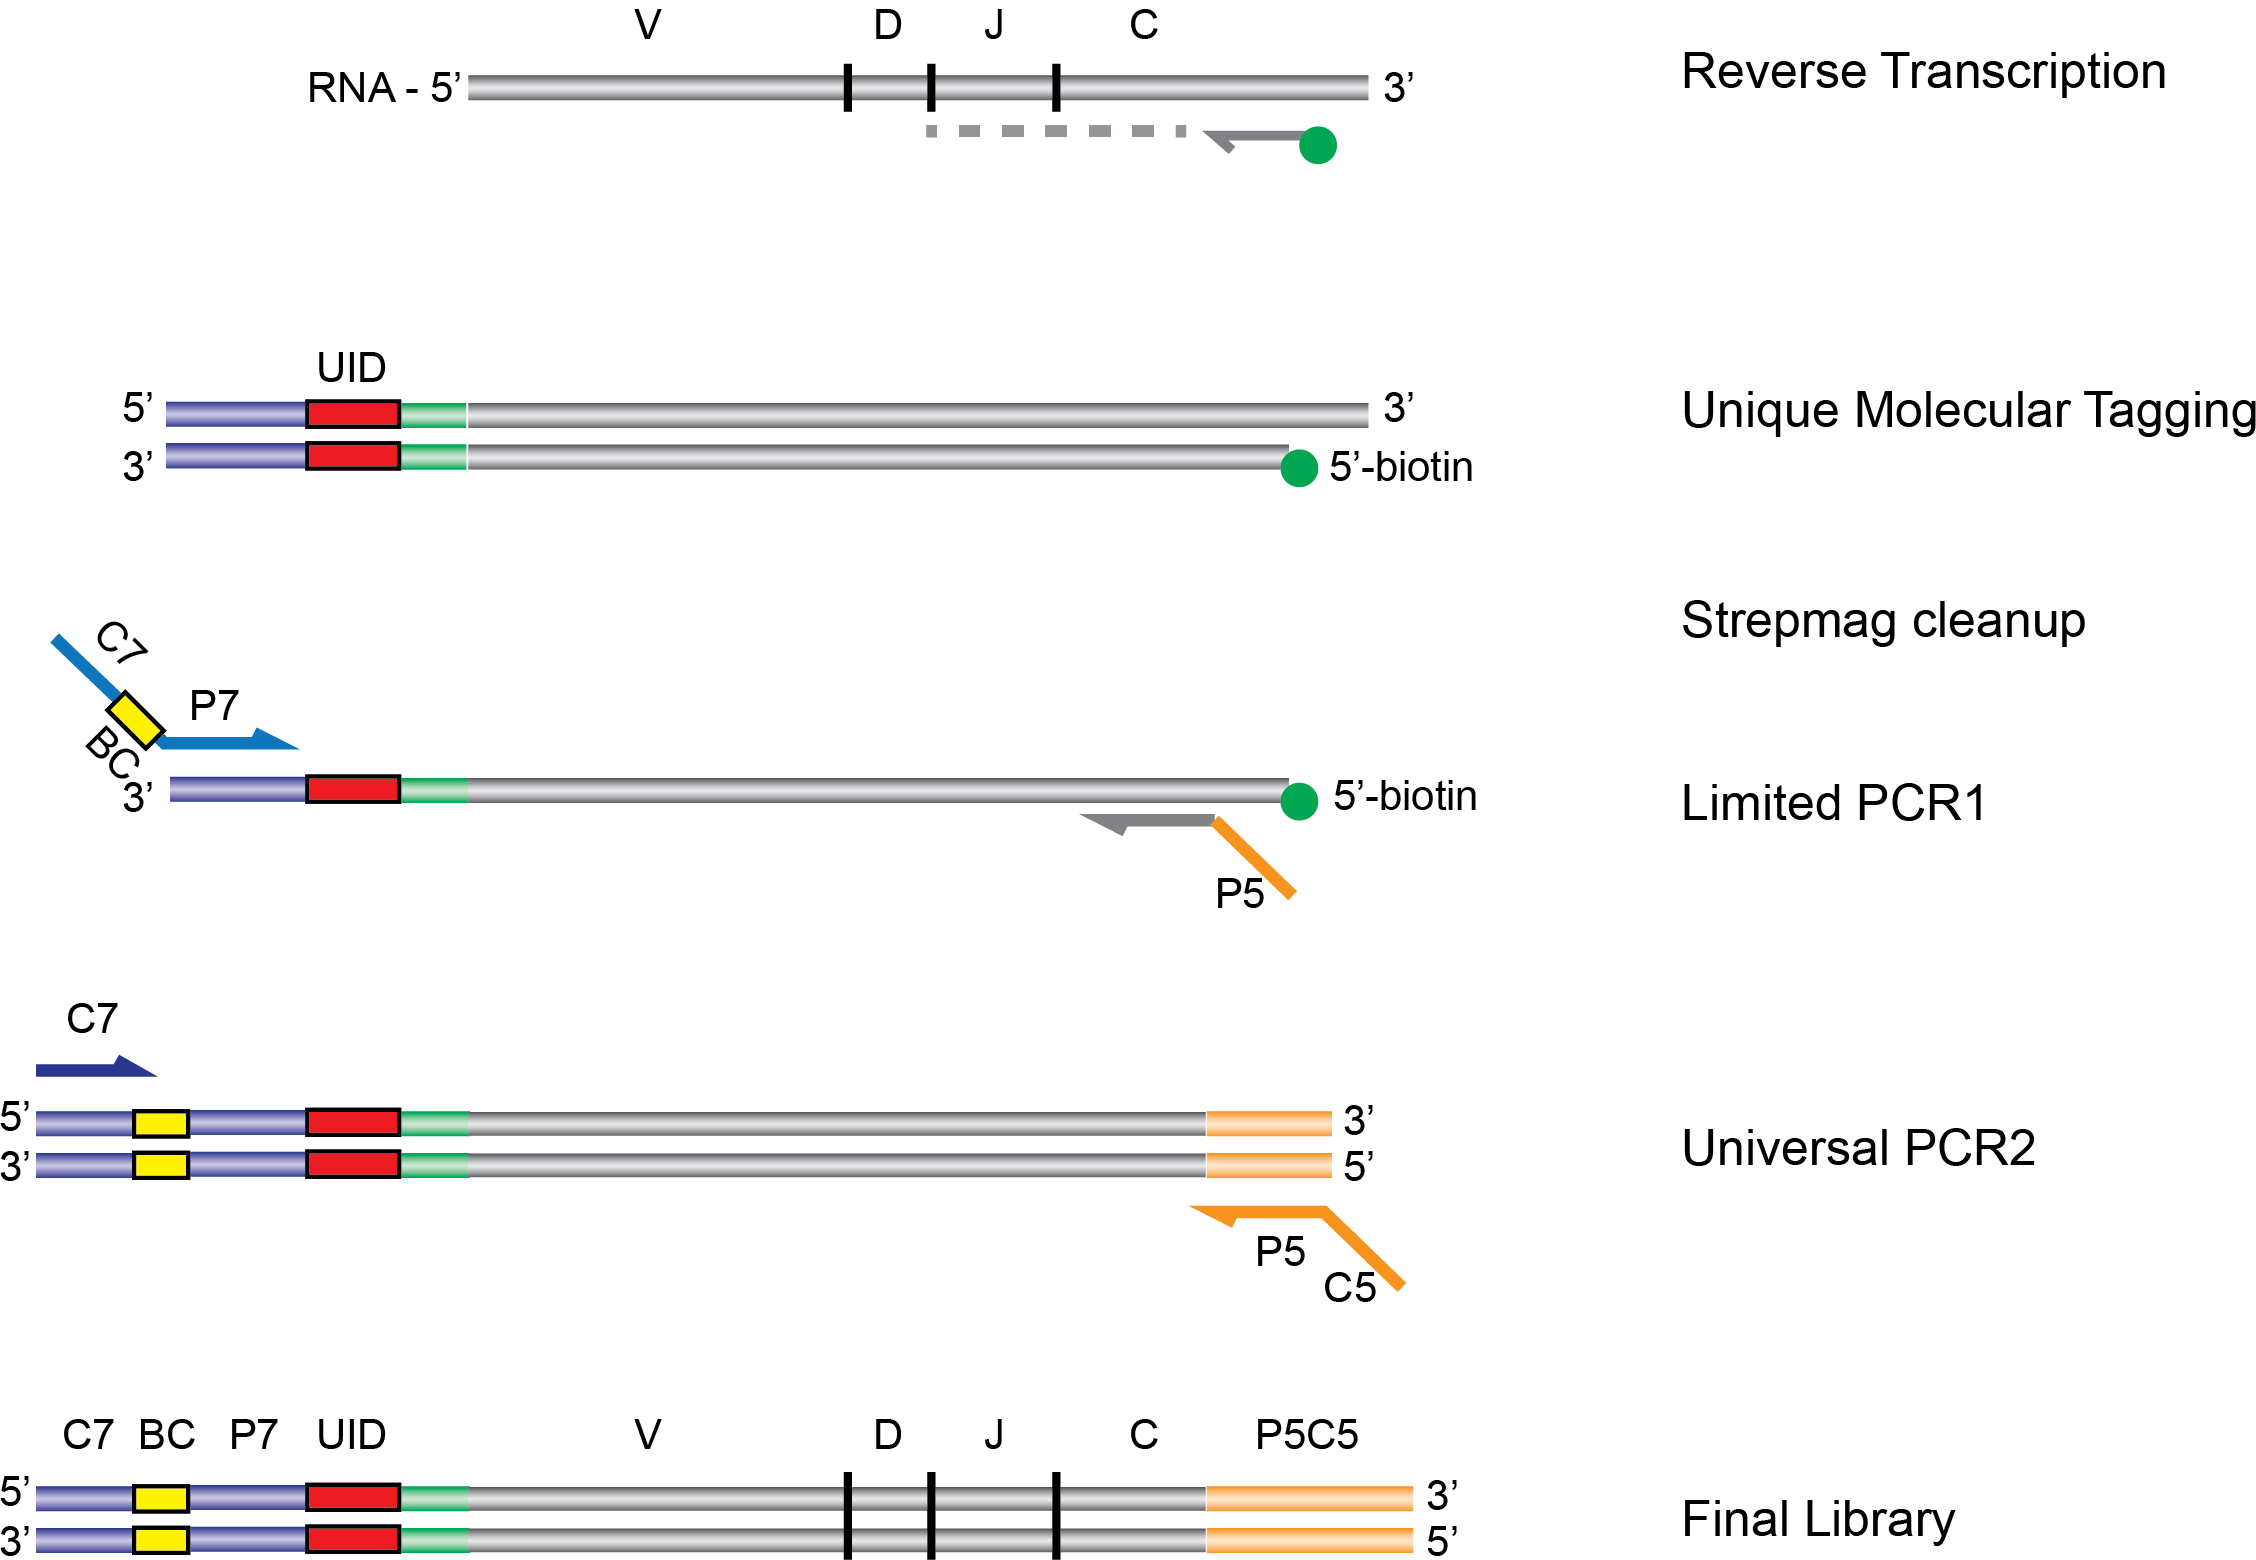
\includegraphics[width=0.8\textwidth]{figures/BCR_RTPCR_AbVitro.png}
    \caption{
        \label{fig:BCR_RTPCR}
        DNA prep method for BCR sequencing on Illumina developed and used by AbVitro (now Juno Therapeutics).
        In the first step an RT-PCR is run with template switching to introduce a UID.
        The fragments are then purified and the Illumina C7 clustering sequence, and barcode (BC), are attached to the 5'-end.
        Finally the C5 clustering sequence is attached and the library is ready for Illumina paired-end sequencing.
        A similar (but not identical) DNA prep method was used in Stern et al.\ \cite{stern2014b} with figure \ref{fig:UMIread} showing the resulting data format.
        Figure from Laustsen et al.\ \cite{laustsen2017exploration}.
    }
\end{figure}

An effective way to minimize errors introduced by the several steps of RT-PCR, PCR and sequencing is to attach a short unique molecular barcode (UMI, also known as unique identifier or UID) to the end of each read already at the RT-PCR step \cite{turchaninova2016high}.
With enough random UMIs in the pool chances are extremely low that the same UMI will be incorporated into multiple BCR transcripts.
Therefore each UMI will represent a single BCR transcript from the unamplified pool of mRNA, and reads with the same UMI should therefore be identical in the rest of the read.
Conversely reads with different UMIs can have identical BCR sequences because a single cell can, and likely will, have multiple copies of the same BCR transcript.
UMIs therefore also provide a way of transcript level quantification on top of its error correction.

Once the read library has been prepared sequencing is undertakes, usually either on Roche 454, or Illumina MiSeq.
In the early days of Rep-Seq the advantage of Roche 454 was its long read length that could be adjusted to span the entire V gene, and additionally going all the way into J when a short CDR3 appeared.
However with the development of the 2x300bp Illumina MiSeq paired-end reads, see figure \ref{fig:UMIread}, the 454 is out phased in favor of higher throughout and better read quality with much lower chance of indel calling.

\begin{figure}
    \centering
    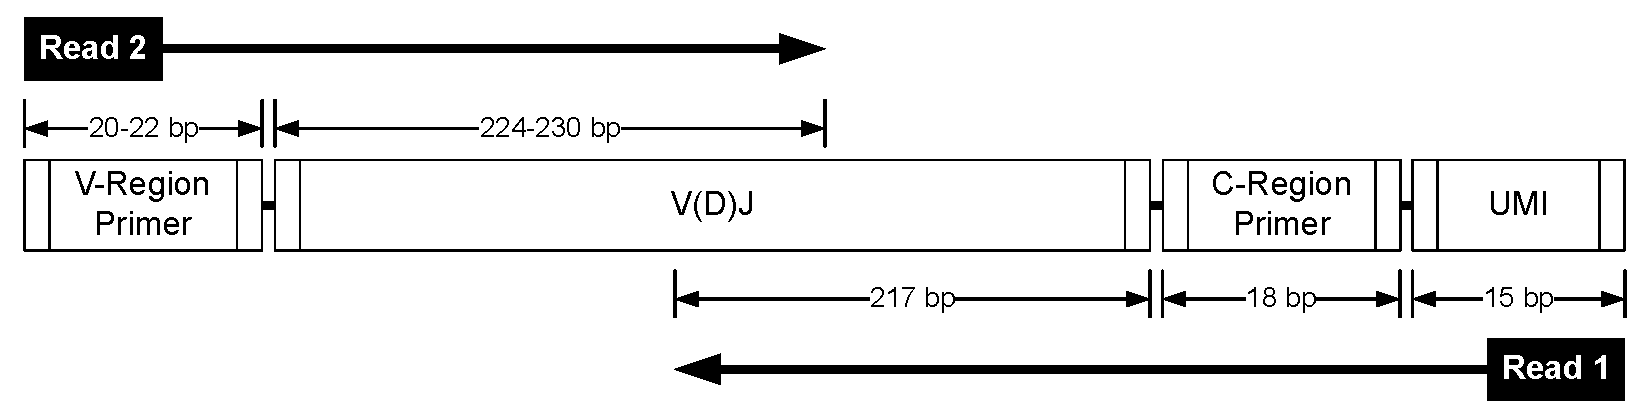
\includegraphics[width=1\textwidth]{figures/Stern2014_ReadConfiguration.pdf}
    \caption{
        \label{fig:UMIread}
        Example of a sequencing strategy for sequencing the full variable BCR chain and parts of the constant region. The strategy is designed for Illumina paired-end reads and seen used in Stern et al.\ \cite{stern2014b}. Figure from pRESTO readthedocs \cite{vander2014presto}.
    }
\end{figure}

After DNA reads have acquired from sequencing, error correction becomes a substantial issue.
In the normal uses of high throughput sequencing, errors are just averaged out by the use of consensus sequences, but in the case of BCR sequencing the inherent variability of the BCR makes it difficult to tease apart what DNA variations that can be attributed to SHM and junctional diversity, and which can be attributed to PCR and sequencing errors.
With the many different sequencing protocols there can also be large differences in the data processing afterwards, but pipelines exists that are fairly generic and will handle a wide range of data.
A commonly used pipeline capable of processing a wide range of data is pRESTO (\url{presto.readthedocs.io}) \cite{vander2014presto}.
Data processing with pRESTO is still sequencing protocol dependent but largely flexible and funnels down the data into the same end point regardless of protocol.
In the case of paired-end Illumina reads with UMIs, similar to figure \ref{fig:UMIread}, the workflow can be summarized by the flowchart in figure \ref{fig:UMIread_flow}.
Input data is paired-end reads with Phred quality scores in fastq format.
The data quality is first assessed by running FastQC \cite{andrews2010fastqc}, then bad reads are removed or ends are trimmed to sufficient minimum quality.
Many DNA prep protocols are using degenerate primers for PCR amplification by binding to the 5'-end of all possible V genes, see figure \ref{fig:UMIread}.
This will possibly introduce what will look like a mutation, but in fact is a PCR artifact due to promiscuous primer binding.
These should be removed by trimming off the primer binding region or "masking" it by reverting these mutations back to germline (red in figure \ref{fig:UMIread_flow}).
Then the paired-end sequences are merged by merging on the overlapping stretch of read 1 and 2 using simple alignment score maximization.
Read pairs that failed to merge are discarded but the reads are still kept in separate files to build a consensus sequence over the sequences with the same UMI.
Then anther instance of pairing is done on these consensus sequences to synchronize the files followed by merging reads into the same file (orange and green in figure \ref{fig:UMIread_flow}).
Next a series of filtering and deduplication steps are undertaken e.g.\ only allowing sequences with multiple reads, a maximum number of ambiguous nucleotides etc. to pass through.
The final result should be a set of high confidence BCR sequences, and depending on the sequencing protocol, with or without information about the constant region and/or mRNA abundances.

\begin{figure}[ht]
    \centering
    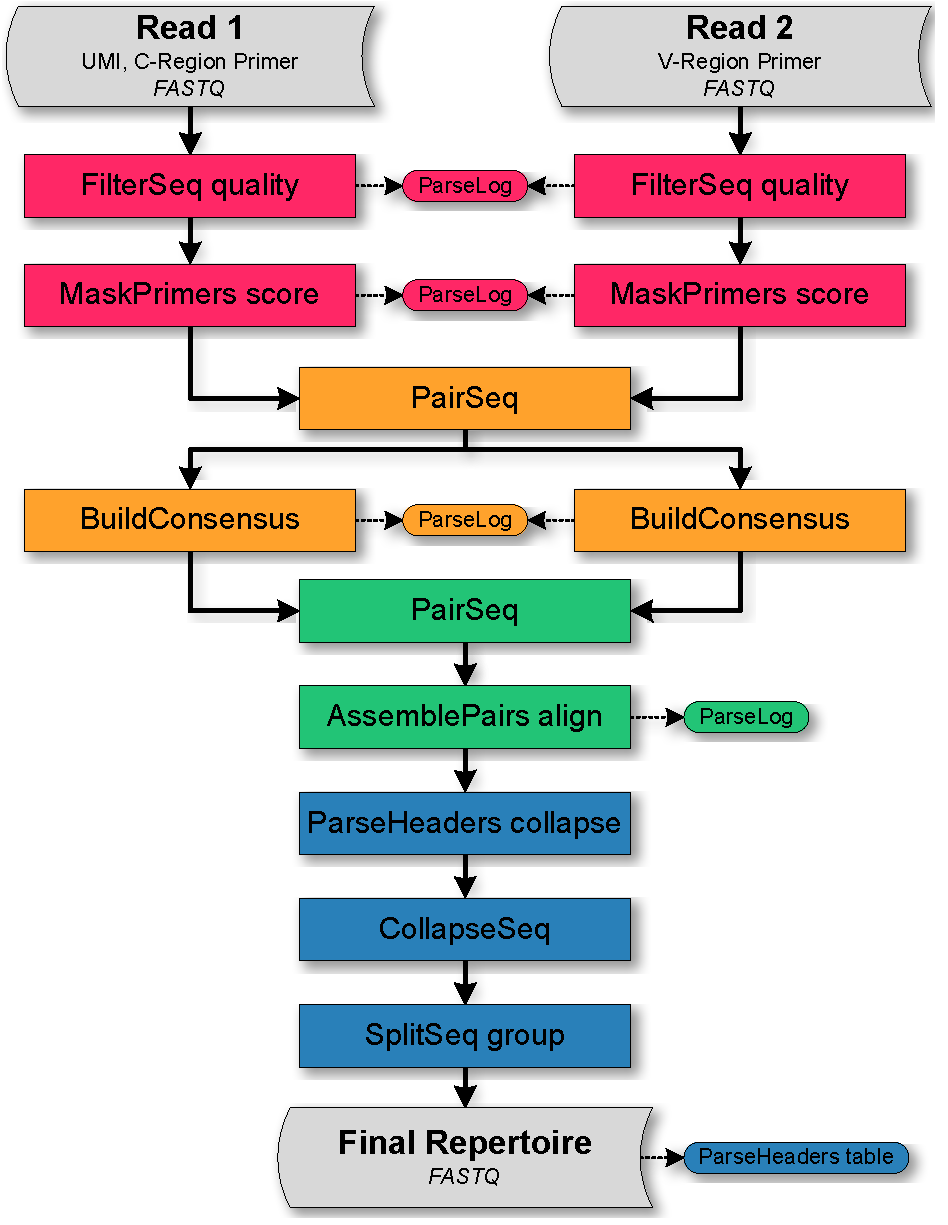
\includegraphics[width=0.55\textwidth]{figures/Stern2014_Flowchart.pdf}
    \caption{
        \label{fig:UMIread_flow}
        Flow of the raw sequencing data through the pRESTO pipeline. This strategy is designed for Illumina paired-end reads, e.g.\ \ref{fig:UMIread}, and seen used in Stern et al.\ \cite{stern2014b}. From pRESTO readthedocs \cite{vander2014presto}.
    }
\end{figure}


All of the above described sequencing methods suffer under the substantial caveat that they are mixing the heavy and light chain sequences from multiple cells under the mRNA isolation step.
This means that a given heavy chain sequence could have been paired with any of the light chain sequences observed for the same sample - and with high throughout sequencing this is millions.
Pairing is not always necessary e.g.\ in some cases of diagnostics, but if the function of an antibody is to be tested the correctly paired heavy/light chain needs to be found.
Some authors have done so using random pairing and selecting for binding via phage display \cite{glanville2009precise}, others have ranked heavy and light chains according to their frequencies from sequencing and matched the highest frequency clones \cite{reddy2010monoclonal}, yet others have used phylogenetics to infer trees and then pair similar topology heavy/light chain trees, guided by a known pair to link to trees \cite{Zhu_undated-zz}, \cite{kwong2017antibodyomics}, \cite{huang2016identification}.
The latest development is to use micro-droplets to capture single cells and then perform the DNA prepping steps inside these drops.
Some authors are pairing heavy/light by physically linking them together via overlap PCR \cite{mcdaniel2016ultra}, while others are amplifying a UMI inside the drop and attaching it to both heavy and light chains \cite{Briggs134841}.
Though the methods for paired heavy/light chain sequencing now exists they are not widely used because of the requirement of having a micro-droplet platform and expert knowledge which is not common stock for most labs.
Still the vast majority of public BCR sequencing data is unpaired and it will likely remain so for at least some years to come.



\subsection{Inferring B cell clonal families}
Once high quality sequences have been obtained from a BCR repertoire sequencing they become the input to the following analysis steps, either as hypothesis testing or hypothesis creating.
A first step in the analysis is simply to annotate sequences by their germline VDJ genes, which can be done simply by aligning each sequence from a database of germline genes to the BCR sequence at hand.
The V, D and J genes achieving the highest alignment score are the winners and inferred to be the true germline gene present on the ancestral naive sequence.
This approach is used by many studies to VDJ annotate BCR sequences, usually either through the NCBI hosted IgBLAST \cite{ye2013igblast} or IMGT's V-QUEST \cite{li2013imgt}.
The advantage of using IgBLAST is its fast turnover and stand-alone software under a permissive license.
Next, an extension to inferring the germline genes is to infer the full naive VDJ sequence of its unmutated ancestor.
Inferring the full naive sequence is a bit more complicated because it requires inferring the original sequence flanking the D gene, where the junctional diversity from N/P nucleotides is complicating the problem.
Given a BCR sequence and assuming some distribution of N/P nucleotide insertion, how many bases is trimmed of the V-D junction and how many are trimmed of the D-J junction?
%Assuming uniform randomly inserted N/P nucleotides nothing can be inferred other than the 25\% chance of either of the bases, however the problem is how many bases is trimmed of the V-D junction and how many are trimmed of the D-J junction?
This question is non-trivial because of SHM e.g.\ if a single mismatch is preventing a V gene alignment match to extend further 4 bases downstream, see table \ref{extend_or_not}, should that be regarded as a mutation due to SHM, or is it regarded as the last 3 random N/P nucleotides incidentally had the same identity (uniform random chances $0.25^3=0.0156$)?
Clearly it looks like an extension to the alignment would be the optimal solution but what then if the last base was also a mismatch? Or that about the effect of the underlying distribution of N/P nucleotide insertions?
In these complex cases intuition starts breaking down, instead there is need for a statistical model that can integrate over probabilities and give consistent estimates.
\begin{table}[ht]
\centering
\begin{tabular}{l}
\texttt{V gene \ ...GTTGAGTGT} \\
\texttt{\ \ \ \ \ \ \ \ ...|||||*|||} \\
\texttt{BCR seq ...GTTGAATGT}
\end{tabular}
\caption{To extend, or not to extend, that is the question (for an HMM to answer).}
\label{extend_or_not}
\end{table}

The classical "go to" statistical model for biological sequence analysis is a hidden Markov model (HMM) \cite{durbin1998biological}.
Briefly an HMM is set of user defined states, e.g.\ the V, D or J genes, N/P insertions, etc., and the jump between states are then connected by probabilities.
Each state has a list of emission probabilities that defines the probabilities of observing a given base.
%There is also a probability of changing state e.g.\ from V gene to N/P insertion.
The hidden/unknown part is the identity of the states at a given position in a sequence e.g.\ when is the V gene stopping and the N/P insertion starting, like the example above.
This is one of the question that is possible to answer using an HMM, specifically by calculating the so called Viterbi path, but what is more interesting is the inherent flexibility of an HMM to represent well known biological mechanisms in a statistical framework.
% It is out of the scope of this work to explain the inner workings of HMMs, how to find the optimal path, estimating parameters etc.
% For this the book by Durbin et al.\ \cite{durbin1998biological} is an excellent resource.

To address the problem of BCR sequence annotation Ralph et al.\ developed an HMM model of VDJ recombination and built it into a software called partis \cite{ralph2016consistency}.
Using extensive simulation studies, the authors observed clear shortcomings of the purely alignment based method like IgBLAST and IMGT V-QUEST.
Especially, alignment based methods appeared to have a low fraction of correct gene calls for the short germline genes D and J carrying a few mutations, see figure \ref{fig:partis_Jgene_comparison}.
The length of the V gene makes it easy to correctly assign just by alignment, and therefore little performance difference was observed, however notice that this only applies for correctly calling the gene identity, regardless of allele identity.
With the more subtle variations among the alleles, there probably is an even bigger performance gain here, by using HMMs like partis compared to pure alignment based methods.

\begin{figure}
    \centering
    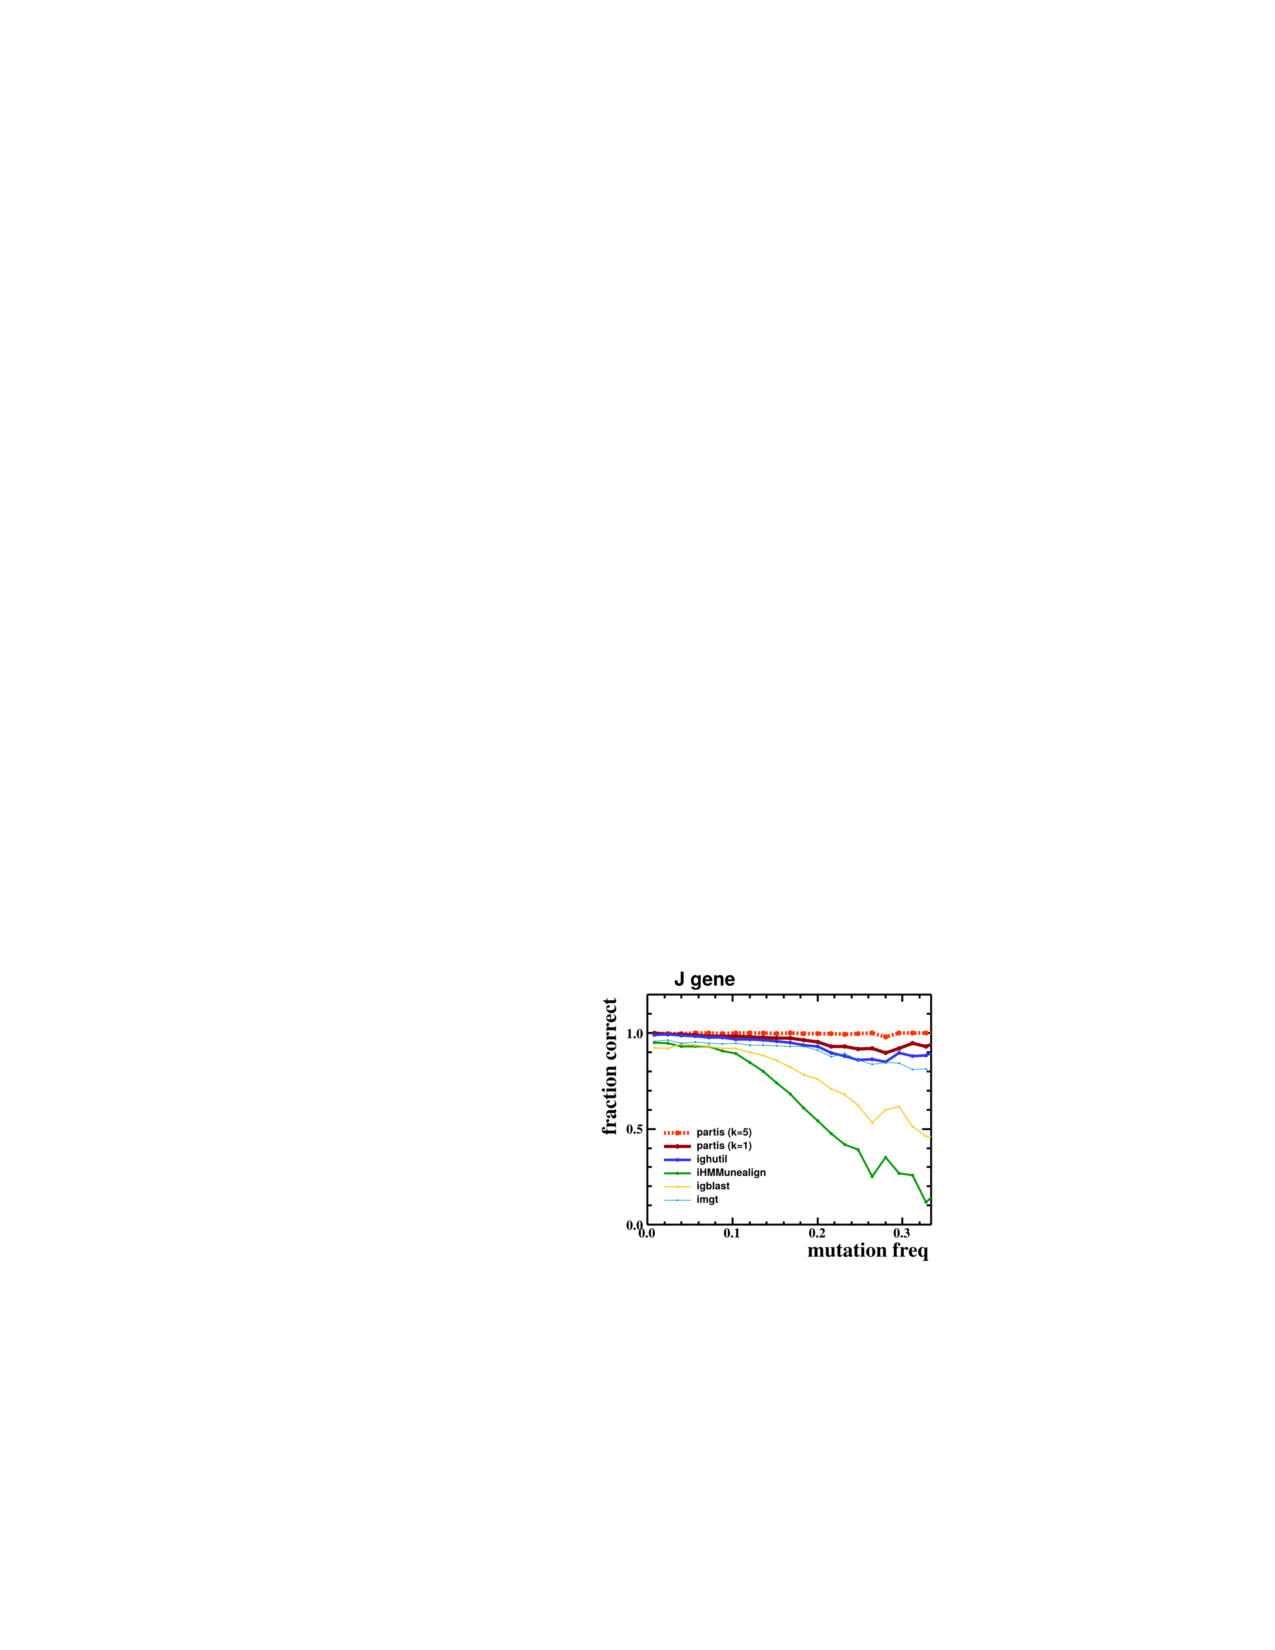
\includegraphics[width=0.5\textwidth]{figures/partis_Jgene_comparison.pdf}
    \caption{
        \label{fig:partis_Jgene_comparison}
        J gene assignment performance for different methods.
        With higher mutational burden most methods struggle to make the correct gene assignments, presumably because of the problem outlined in table \ref{extend_or_not}.
        The HMM method in partis is robust to the mutation burden, and achieves even higher performance by integrate over multiple (k=5) sequences from the same clonal family.
        IHMMunealign and partis are the only HMM methods while the rest are alignment based.
        From \cite{ralph2016consistency}.
    }
\end{figure}


Now returning to the alignment problem exemplified in table \ref{extend_or_not}.
The real shortcoming of using a pure alignment methods is that there is no robust way of deciding what is N/P nucleotides and what is inherited from germline genes, thereby making it very difficult to reconstruct the true naive sequence.
A problem that is well handled by an HMM which will also, as a side effect of calculating the Viterbi path, return the maximum likelihood estimate of the naive sequence.
The speculations were confirmed in the simulation study of Ralph et al.\ that showed substantial performance gains in naive sequence reconstruction using HMMs vs.\ alignment methods, see figure \ref{fig:partis_naiveseq_comparison}.

\begin{figure}
    \centering
    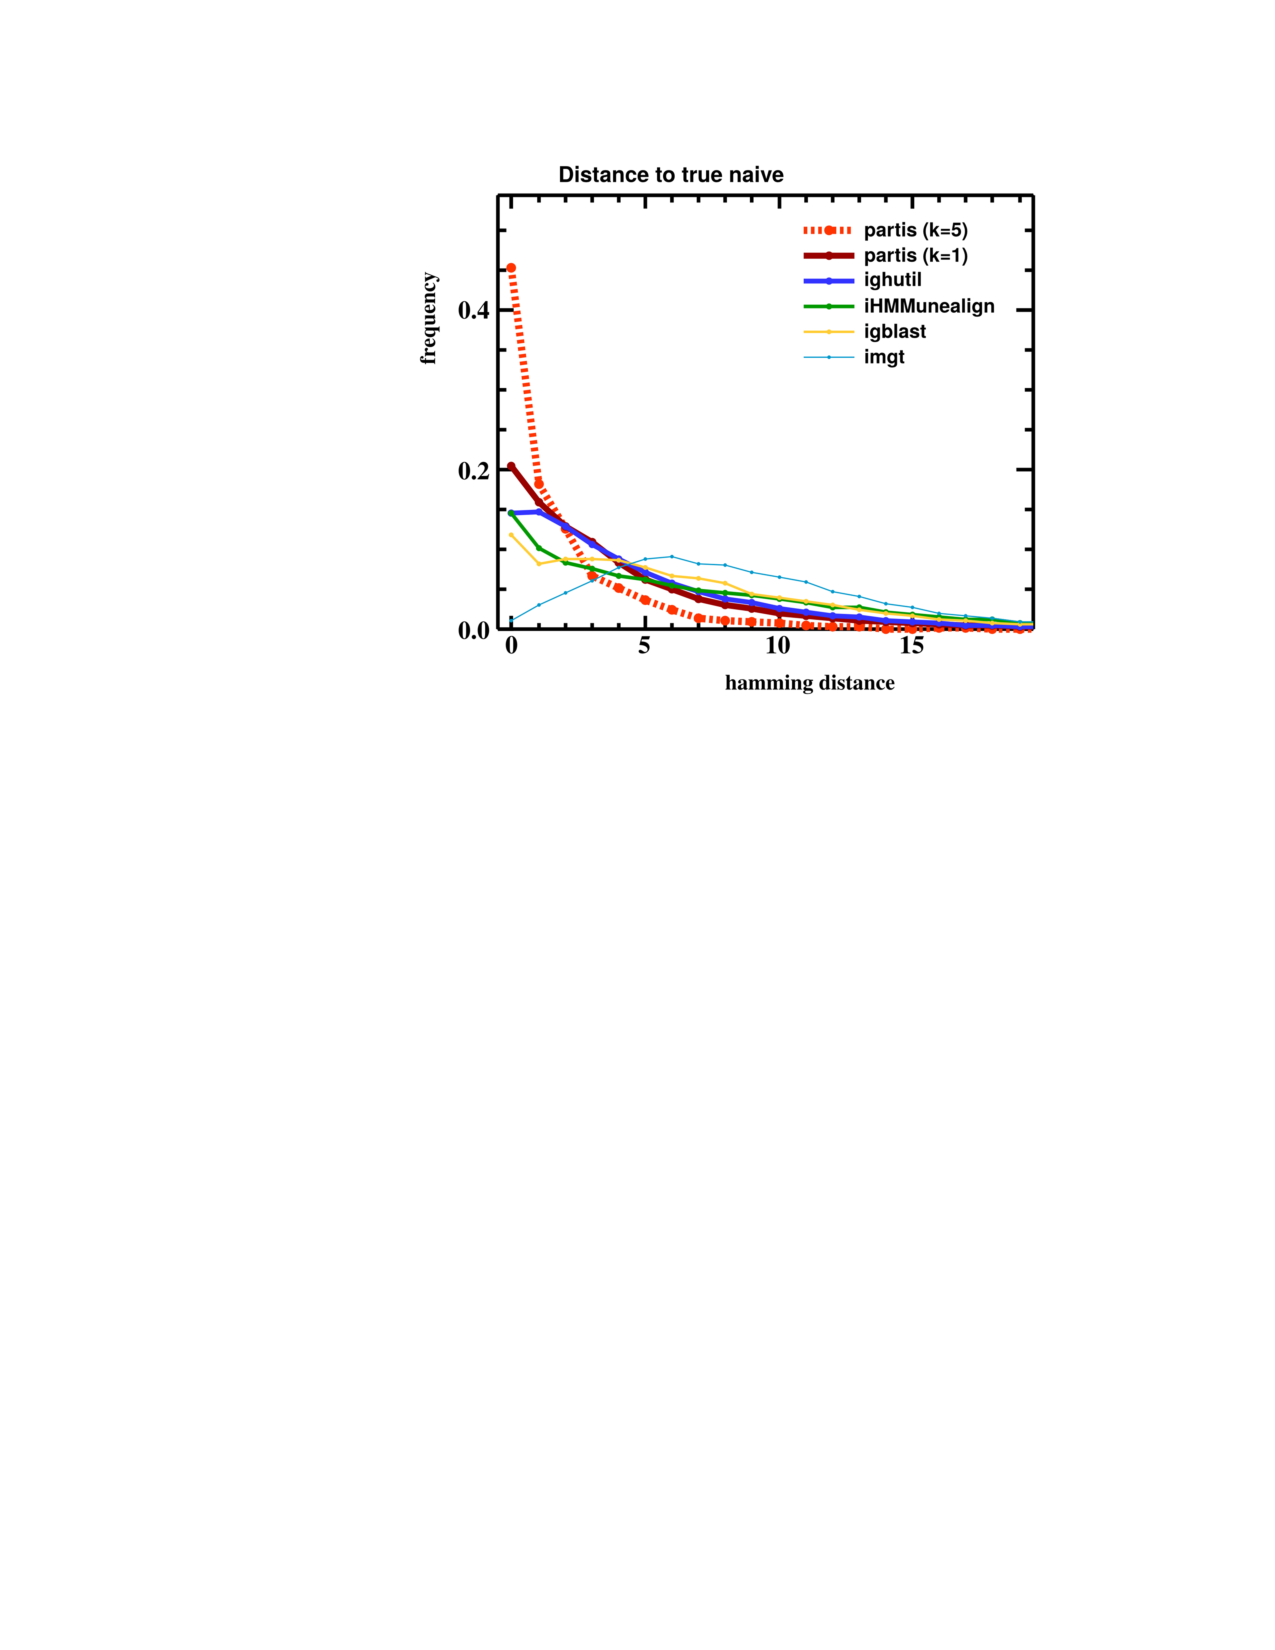
\includegraphics[width=0.5\textwidth]{figures/partis_naiveseq_comparison.pdf}
    \caption{
        \label{fig:partis_naiveseq_comparison}
        Distribution of hamming distances true vs.\ inferred for 30,000 simulations compared across different inference methods.
        There is a clear advantage of using HMM methods like partis, but the largest performance leap is to integrate over multiple (k=5) sequences from the same clonal family (explained in the clustering section).
        IHMMunealign and partis are the only HMM methods while the rest are alignment based.
        From \cite{ralph2016consistency}.
    }
\end{figure}


Next step is to partition the BCR sequences into clusters of sequence related by some definition of relatedness.
These clusters are by some known as clones \cite{gupta2017hierarchical}, which is assumed to mean that they actually came from the same GC reaction.
However as previously discussed the view of GCs as monoclonal is outdated \cite{tas2016visualizing}, so in this work the nomenclature from Ralph et al.\ \cite{ralph2016likelihood} is used, with the assumption that there is sufficient BCR diversity to distinguish clonal families exclusively based on their shared naive sequence.
% Nevertheless the biologically interpretation is that all the sequences in a cluster are highly similar and share the same epitope for binding.
Given this definition a logical first step would be to require that the assigned germline genes in a cluster to match, and indeed such simple clustering has been extensively used.
However in acknowledgement of the uncertainty in assigning the correct D gene, only V and J genes are usually used, and regardless of their allelic variants.
Furthermore the junction length or the CDR3 length has been used as second discriminator and the hamming distance between sequences is usually used as the last discriminator.
Then the procedure for clustering is first to split BCR sequences into buckets with the same V and J gene and junction or CDR3 length, and then sequences in each bucket are clustered based on a distance measure like hamming distance \cite{glanville2011naive}, SHM weighted hamming distance \cite{gupta2017hierarchical} or amino acid based hamming distance confined to CDR3 \cite{jiang2013lineage}.
This method, which will be referred to as "VJ junction agglomeration", has the inherent problem of putting 100\% confidence on the V, J and junction annotations.
However with just moderate SHM there are substantial uncertainties in the annotations and in such cases putting a hard boundary between sequences with different annotations causes problems.
In an example, outlined in figure \ref{fig:VJ_CDR3_agglomeration}, a clonal family would wrongly be assigned into three different clusters (boxes defined by the solid gene lines) if VJ junction agglomeration is used.
Contrarily, if integrating over germline and junctional annotation uncertainties, clustering is not restricted by the point estimate of the gene or allele annotation, and at least has the possibility to merge all red dots into the same cluster.

\begin{figure}[ht]
    \centering
    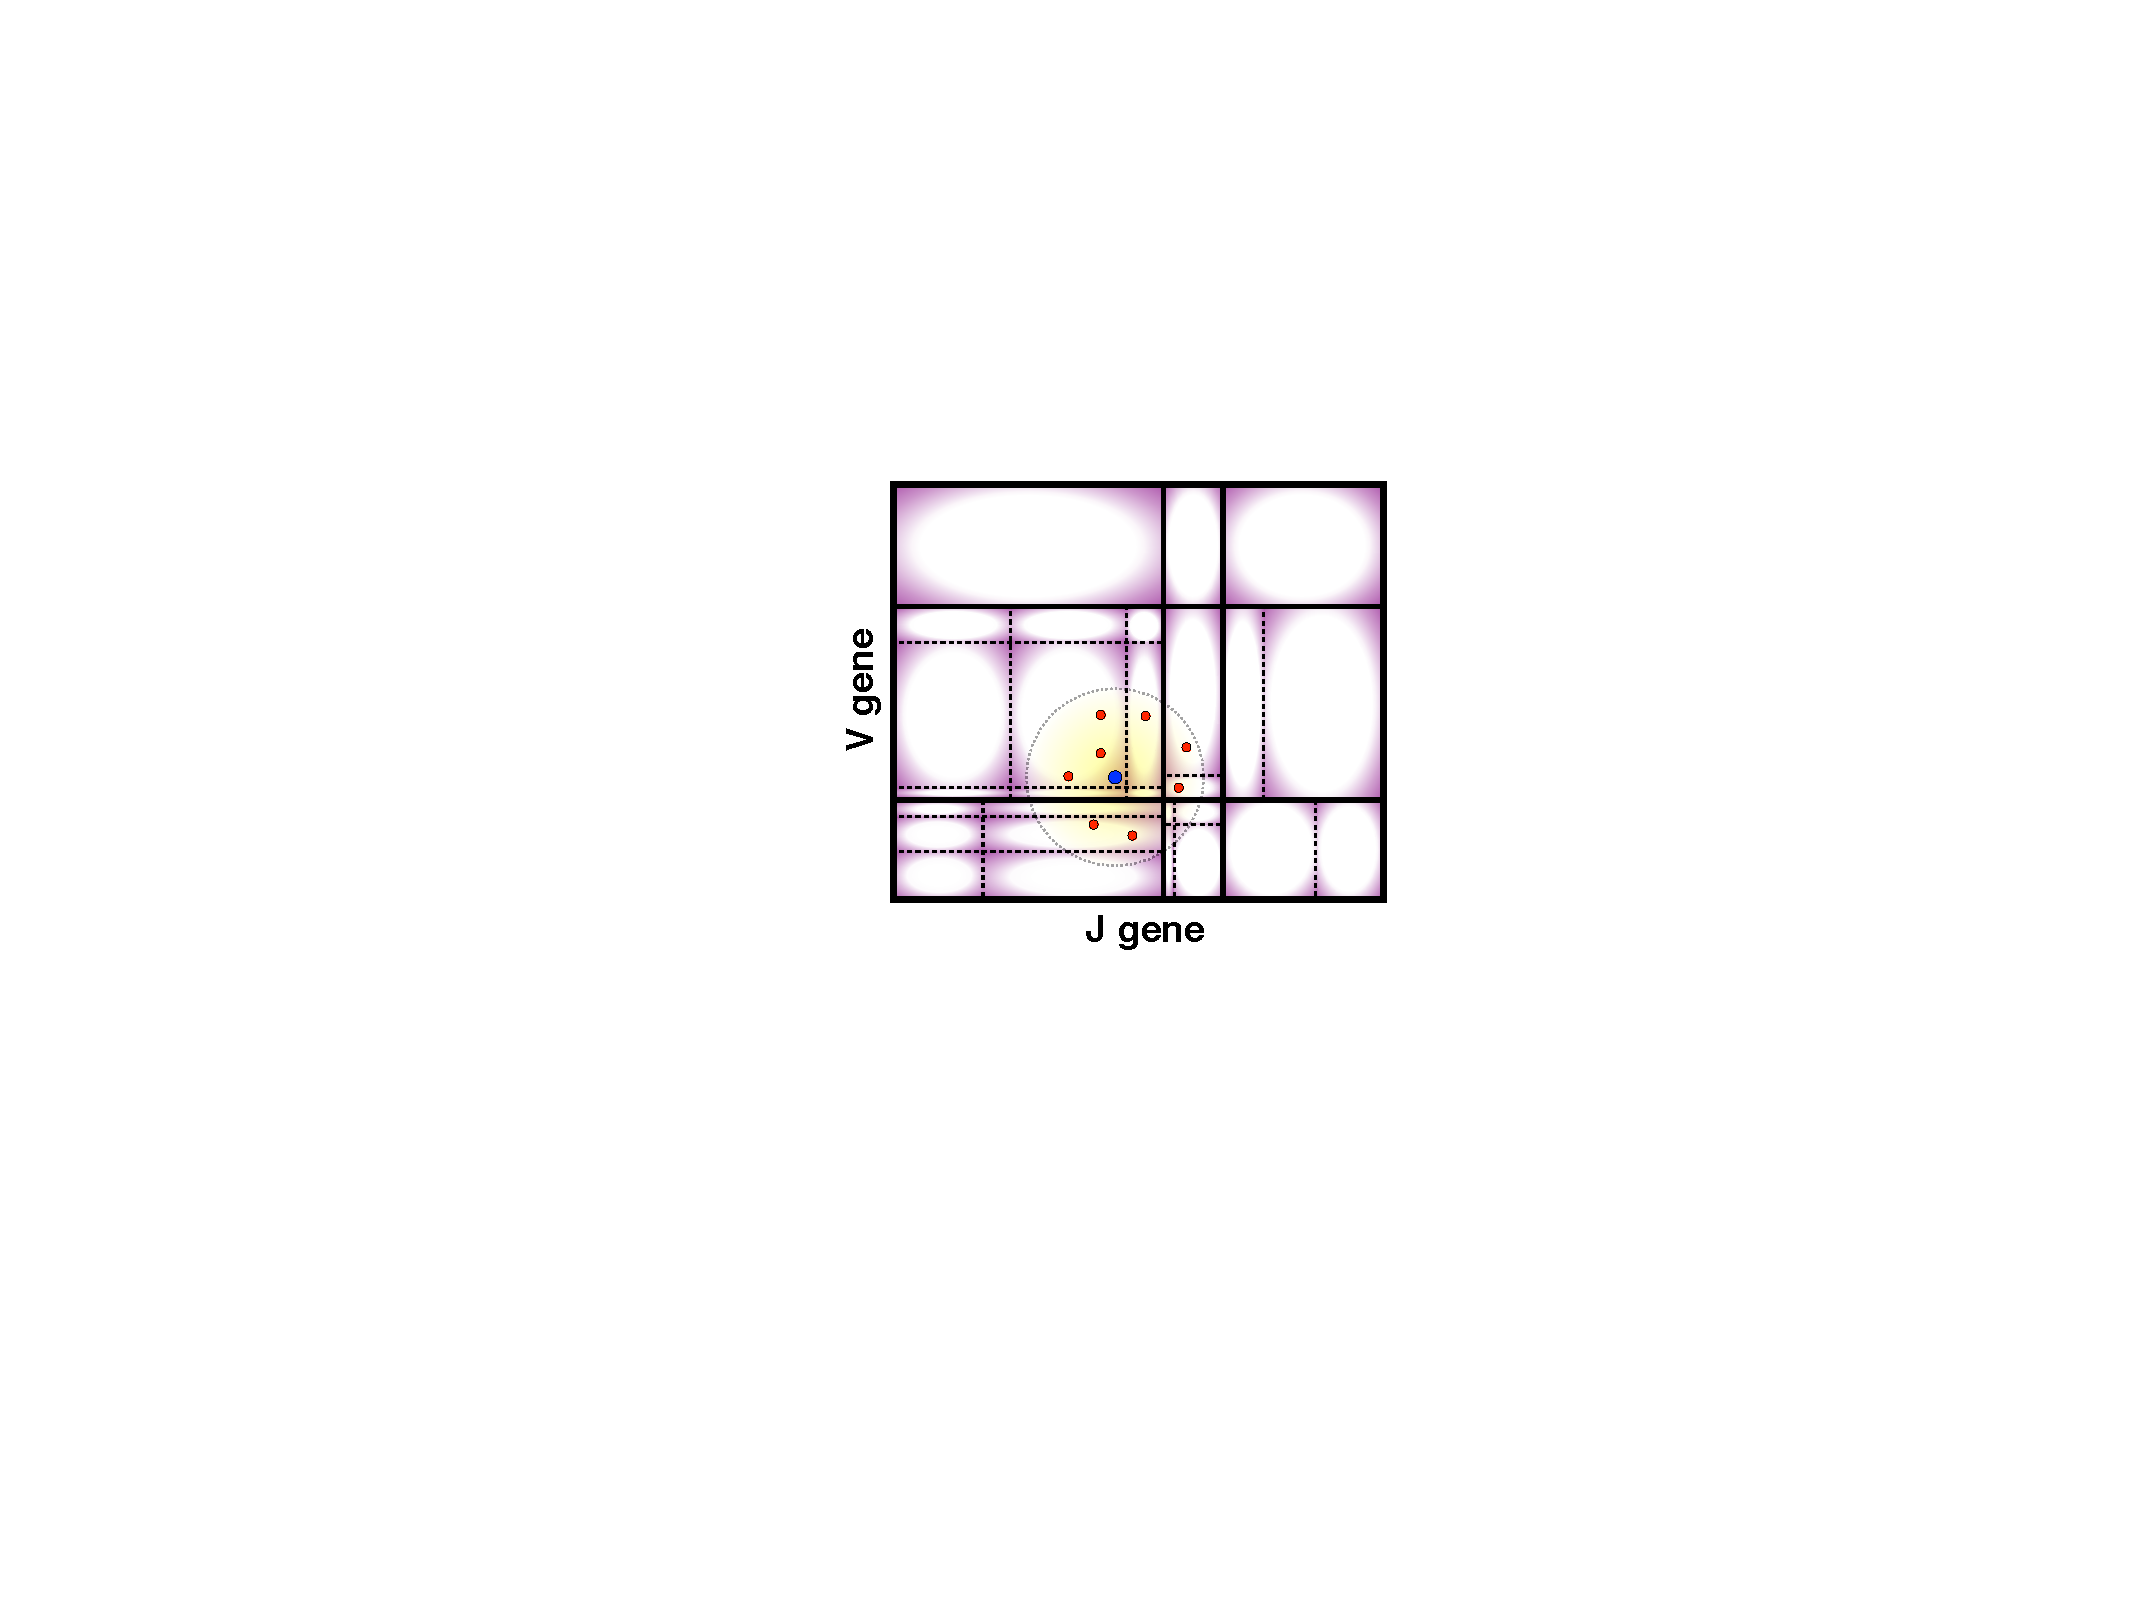
\includegraphics[width=0.5\textwidth]{figures/VJ_CDR3_agglomeration.pdf}
    \caption{
        \label{fig:VJ_CDR3_agglomeration}
        Two dimensional representation of the BCR sequence space that illustrates how V, J and junction point estimates leads to overestimation of the number of clusters.
        Vertical lines represent V genes and dashed lines represent alleles, same for J genes on the horizontal axis.
        Naive sequences with no N/P nucleotides are in the cross section between a V and J allele.
        Colored with purple gradient is the range of junctional diversity extending from the V/J gene combinations, less color means lower probability, all the way to white which is sequences not within the reach of any VDJ recombination.
        The dot in blue represents a naive sequence with its SHM "breadth" marked by a yellow circle.
        Red dots are observed BCR sequences from the clonal family defined by the naive sequence.
    }
\end{figure}


Now it should be clear that the root cause of the clustering problem is propagation of errors in point estimates, i.e.\ ignoring the substantial uncertainty in VDJ annotations of a BCR sequence that has undergone SHM.
When a clustering criterion is based on the point estimate of both the V and J assignment, both the assignment uncertainties are affecting the clustering performance negatively.
The junction length is also problematic to use because it is also just a point estimate, and often estimated from by a problematic alignment method as outlined in the example in table \ref{extend_or_not}.
Lastly, hamming distance is weighting a mismatch in the N/P base region equally likely as a mismatch in the middle of germline gene while there is much more certainty of a real SHM event in the later case.
In the example in figure \ref{fig:VJ_CDR3_agglomeration} VJ junction agglomeration is overestimating the number of clusters and indeed this intuition is also observed in simulation studies \cite{ralph2016likelihood}.

A completely different approach is taken by Ralph et al.\ \cite{ralph2016likelihood}, extending on their HMM framework for germline gene annotation.
They use the naive sequence as a centrality point for clustering, not in terms of hamming distance, but in the terms of likelihood.
The HMM model is conveniently yielding a likelihood function defined over all possible naive sequences for each BCR sequence in the dataset.
With this likelihood function it gets simple to do hypothesis testing based clustering e.g.\ to test whether a set of observed BCR sequences all belong to the same cluster through a common naive sequence ancestor, see figure \ref{fig:partis_clustering-with-likelihood_2}.

\begin{figure}
    \centering
    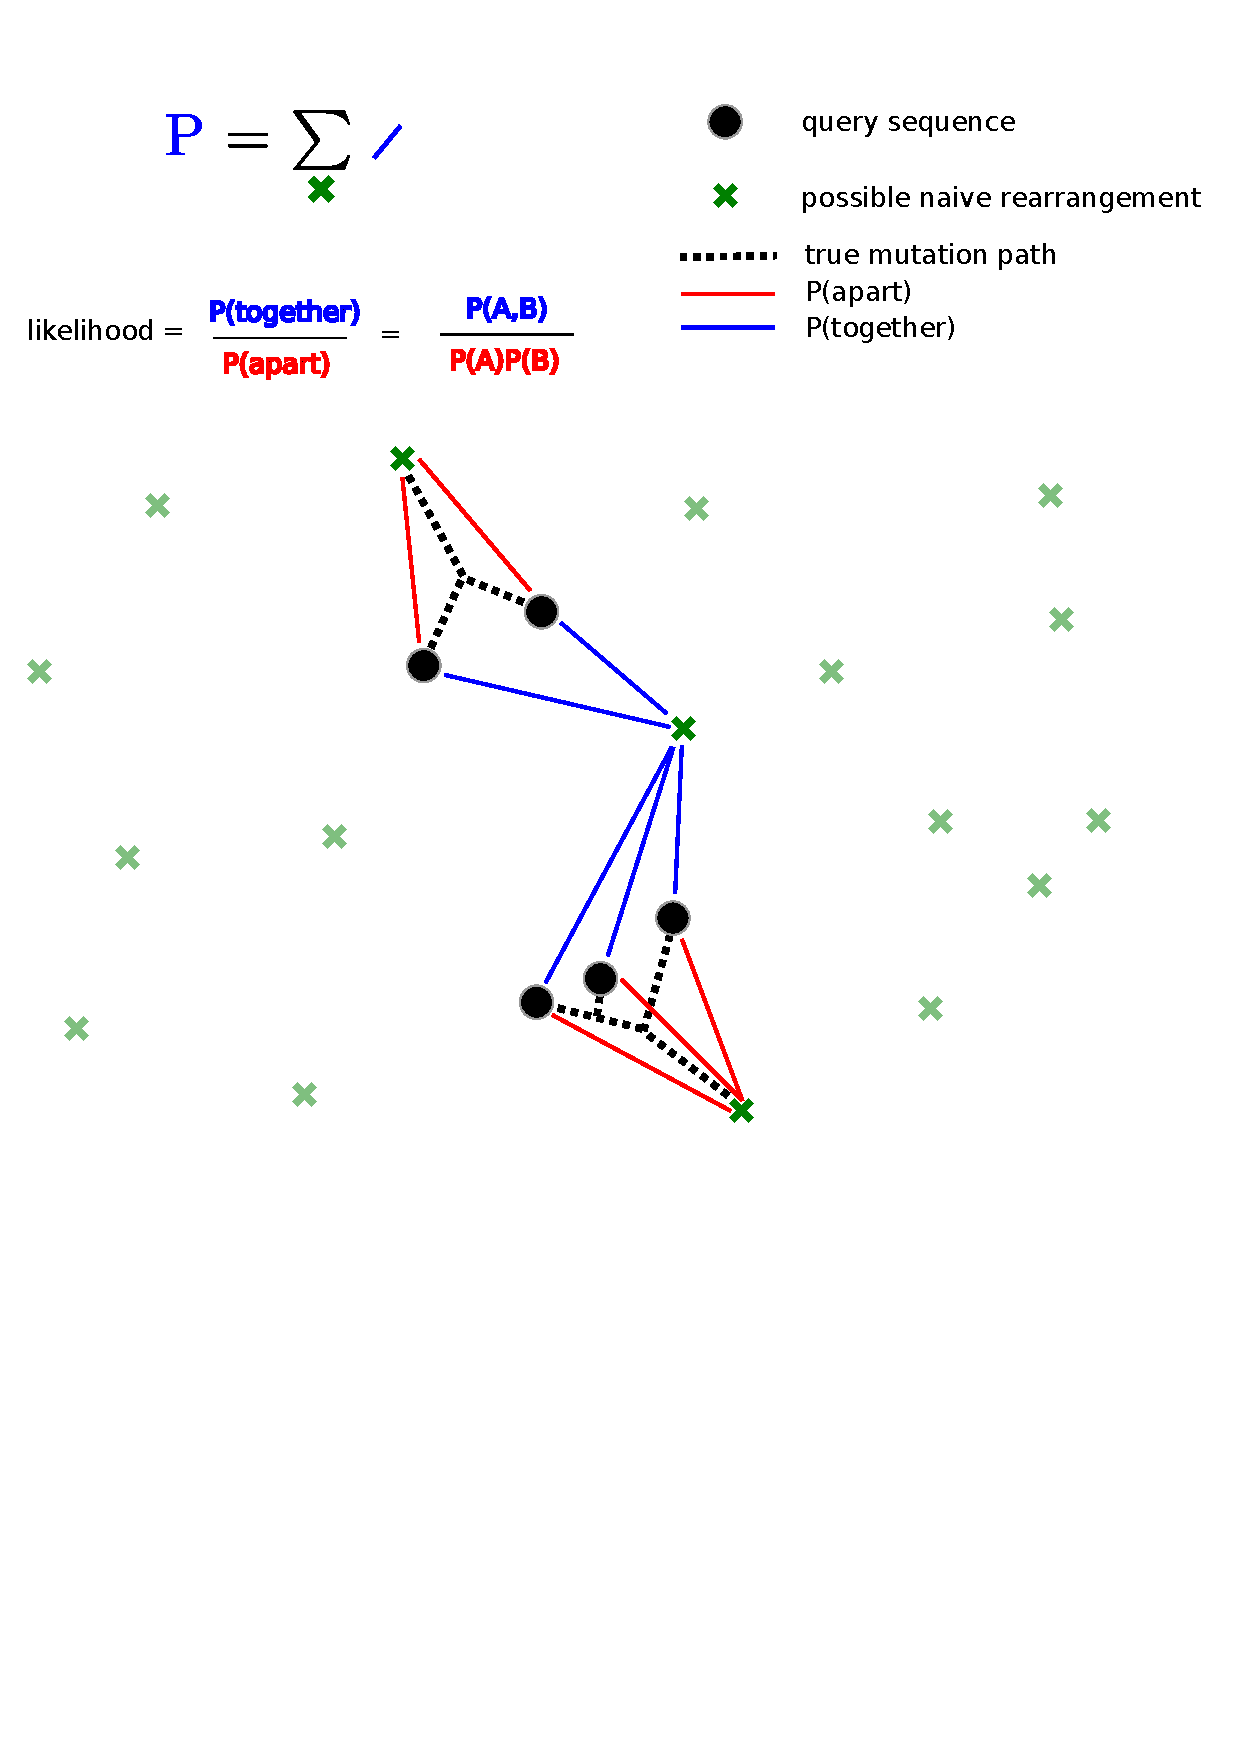
\includegraphics[width=0.7\textwidth]{figures/partis_clustering-with-likelihood_2.pdf}
    \caption{
        \label{fig:partis_clustering-with-likelihood_2}
        Likelihood ratio test to decide whether to merge a set of sequences into a cluster or not. Figure credit: Duncan Ralph.
    }
\end{figure}


Notice that the likelihood ratio test based clustering in partis is centered around the likelihood of the proposed naive sequence and the thus allow for merging of sequences with different VJ gene annotation point estimates.
When clustering has run to an end the final annotation of each sequence will change to reflect a common VDJ rearrangement for all cluster members.
The shared information among cluster members makes inference of the naive sequence much more probable because all sequences can be integrated into the same HMM, referred to as multi-HMM in Ralph et al.
The strength of using multi-HMM to infer a naive sequence is obvious from a theoretical stand-point.
Multiple sequences are regarded as multiple independent observations of the same mutation process and this will increase the probability of the germline annotation, but more so, it will increase the odds of observing the true naive sequence in the N/P junction.
This claim is supported by striking improvement in both annotation (figure \ref{fig:partis_Jgene_comparison}) and naive sequence inference (figure \ref{fig:partis_naiveseq_comparison}) for just 5 clonal family sequences (k=5).

The advantages of HMM based BCR annotation and clustering should now be clear and therefore all germline annotation, naive sequence inference and clustering of BCR sequence throughout this work was done with the partis software (\url{github.com/psathyrella/partis}).











\section{Phylogeny of a clonal family}
The problem of determining phylogenies is the problem of reconstructing the unobserved evolutionary history, usually, using only a sample of states at a single time point.
Since there are no observations of the events prior to the sampling time we cannot be certain about a phylogeny.
The problem turns into an inference problem.
For B cells this translates into finding the evolutionary history starting from a naive B cell, progressing through rounds of SHM in the GC reaction and finally getting sampled at some time $t$.
The only information available is the BCR sequences at the sampling time.

To represent the process of cell division and apoptosis in the GC it is convenient to use a tree.
The root of this tree is the naive B cell, a branching event is a cell division and a terminal leaf is a B cell that have died.
The tree model of evolution is also a useful way of representing relationship among sequences e.g.\ some sequences which are all members of the same tree clade share a common ancestor and most likely are more similar than some other sequence not included in this clade.
The phylogenetic tree should be viewed as a model framework used to describe the evolutionary process, the details that goes into the model framework depends on the problem at hand.



\subsection{Parsimonious tree inference}
Now given that the evolution is following a tree model, the model for inferring the topology must be specified.
A classical method for inference is to maximize tree parsimony.
Motivated by Occam's Razor the best tree is simply the tree that with the fewest changes explain the observed data.
Practically this is done by calculating the tree parsimony score with Fitch's algorithm \cite{fitch1971toward} and then finding the tree with the lowest score.
The parsimony score of a tree ($T$) can be calculated as a sum of all the scores at each site ($p_i$): $S(T) = \sum_{i=1}^m F(p_i | T)$.

With a parsimony score function the possible tree space can be searched and the maximum parsimony (MP) tree can be found.
Tree space can be searched exhaustively only with few taxa but everything above 10 taxa has more than tens of millions of tree making it practically impossible to search exhaustively \cite{felsenstein1978number}.
The branch and bound algorithm is a way of decreasing search space but still finding the best solution \cite{hendy1982branch}, however even with this hill climbing methods have to be used.
In a hill climbing tree search various heuristic tree moves like, nearest neighbor interchange (NNI), subtree pruning and regrafting (SPR) and tree bisection and reconnection (TBR) are used to explore widely around the tree space.

It it clear that the MP method for tree inference is very simple and while this will work in some applications the criterion of maximum parsimony is not strictly how evolution works.
In cases with rate heterogeneity due to a biased mutation processes or selection some sites might evolve much faster than others and this makes the parsimony assumption of equal weight on all substitutions break.
Such complex processes are not accounted for in the MP method making it prone to errors, but even with the simplest sequence evolution process theoretical arguments by Felsenstein have shown that parsimony is inconsistent \cite{felsenstein1978cases}, and since adding parameters to model a complex process is not readily compatible with parsimony, most researchers have turned to model based tree inference.




\subsection{Model based tree inference}
As an alternative to maximizing the parsimony a likelihood function could be formulated to return the likelihood of the data given the tree. Then the problem turns into finding the most likely tree, referred to as the maximum likelihood (ML) tree.
The likelihood function is conditioned on a tree with branch lengths representing distances in a continuous mutation process driven by a mutation rate.% determined by a matrix of substitution rates.
Using gradient decent tree parameters like branch lengths can be adjusted to their ML estimates.
To accommodate more advanced things such as differences in substitution rates, e.g.\ higher rate of \texttt{T->G} than \texttt{T->A}, a rate matrix can be defined.
If the data is at DNA level the rate matrix contains all possible substitutions between DNA characters.
Examples such matrices: the F81 model \cite{felsenstein1981evolutionary} or the widely used general time reversible (GTR) model \cite{tavare1986some}.

DNA substitution models are not aware of protein encoding and therefore does not explicitly discriminate between synonymous and non-synonymous mutations, something that is otherwise crucial for proteins under tight selection.
Therefore it might be useful to translate a DNA sequence into its protein sequence and then use an amino acid substitution matrix like PAM \cite{dayhoff197822}, BLOSUM \cite{henikoff1992amino} or others.
Information is lost in the translation process so if an amino acid model is to replace the DNA model, information loss needs to be outweighed by the gain in performance.
Alternatively a codon model is defined on DNA level, but with DNA level substitutions working on units defined by protein encoding codons.
In this way a codon model will both account for a difference in the rate of synonymous and non-synonymous substitutions and the rate difference between amino acids.
Two popular choices for a codon model are GY94 \cite{goldman1994codon} and MG94 \cite{muse1994likelihood}.



\subsubsection{Bayesian phylogenetics}
In the ML framework both tree, branch length and substitution parameters are all point estimates adjusted to maximize the likelihood function, but point estimates might not always be desirable.
E.g.\ when information like time or rate is to be extracted from a tree then a single point estimate is not very useful because the variance of such estimate is unknown.
Bayesian phylogeny addresses this challenge by integrating over the distribution of trees, branch lengths and substitution parameters by Monte Carlo sampling.
When sampling has converged the resulting posterior distributions of all parameters can be used to express confidence in the maximum a posteriori (MAP) estimate e.g.\ by providing the high density interval (HDI) along with the MAP estimate.
The real drawback of Bayesian phylogeny is that sampling can make runtime much slower than a similar ML problem.
There can also be a problem of reaching convergence in cases where sampling is difficult.





\subsection{Ancestral sequence reconstruction}
As a side result of inferring a phylogeny it is also possible to reconstruct the sequence of those nodes that are internal and unobserved in a tree.
This process is known as ancestral sequence reconstruction (ASR).
For the MP algorithm these ancestral states are part of the tree inference and found via Fitch's algorithm, but for a model based method ancestral sequences must be estimated by extracting the maximum likelihood estimate of the sequence at each internal node.
ASR on ML trees can either be done as a marginal or a joint reconstruction.
In the marginal case each node is reconstructed independently from one another, found as the ML estimate without fixing the sequence of any of the other internal nodes.
Notice that when one ancestral sequence is found this will change likelihood function for the tree and thereby affecting all the other internal node.
This effect is ignored in marginal reconstruction but accounted for in joint reconstruction where the problem is to find the ML estimate of all the ancestral sequences jointly.

ASR is an important way of exploring the evolutionary trajectory and behaviour of ancient proteins.
It has been used to investigate the specificity of the important cancer drug type kinase inhibitor \cite{Wilson2015-vi} and studying evolutionary trajectories of broadly neutralizing HIV antibodies \cite{Doria-Rose2014-vi}.
Yet there has been little validation of ASR methods partly because it is difficult to test experimentally.
An exception to this was enabled by a clever study design made by Randall et al.\ \cite{randall2016experimental}, using a controlled system of evolution on a single gene with sampling of ancestors, they could experimentally validate ASR inference methods on the using only the final time point.
Results showed high accurary of 97.17-98.88\% correct reconstruction and only small difference between chosen methods.




\subsection{Genotype collapsed tree}
While B cells in a GC reaction are having a high mutation rate there are still many B cell with the same genotype.
Especially after a clonal expansion many B cells will have the same genotype, and furthermore ancestral B cells might have the same genotype as their descendents.
BCR clonal family sequences are generally of low complexity and not very divergent, but because there are many B cells in a GC their phylogenetic trees are seemingly complex with hundreds to thousands of taxa.
To reduce this complexity we use the concept of a genotype collapsed tree (GCtree).
In a GCtree B cells with the same genotype are merged into a single node carrying their total abundance and a leaf descending from a B cell with the same genotype is merged upwards, see figure \ref{fig:GCtree_illu}.

\begin{figure}[!ht]
    \centering
    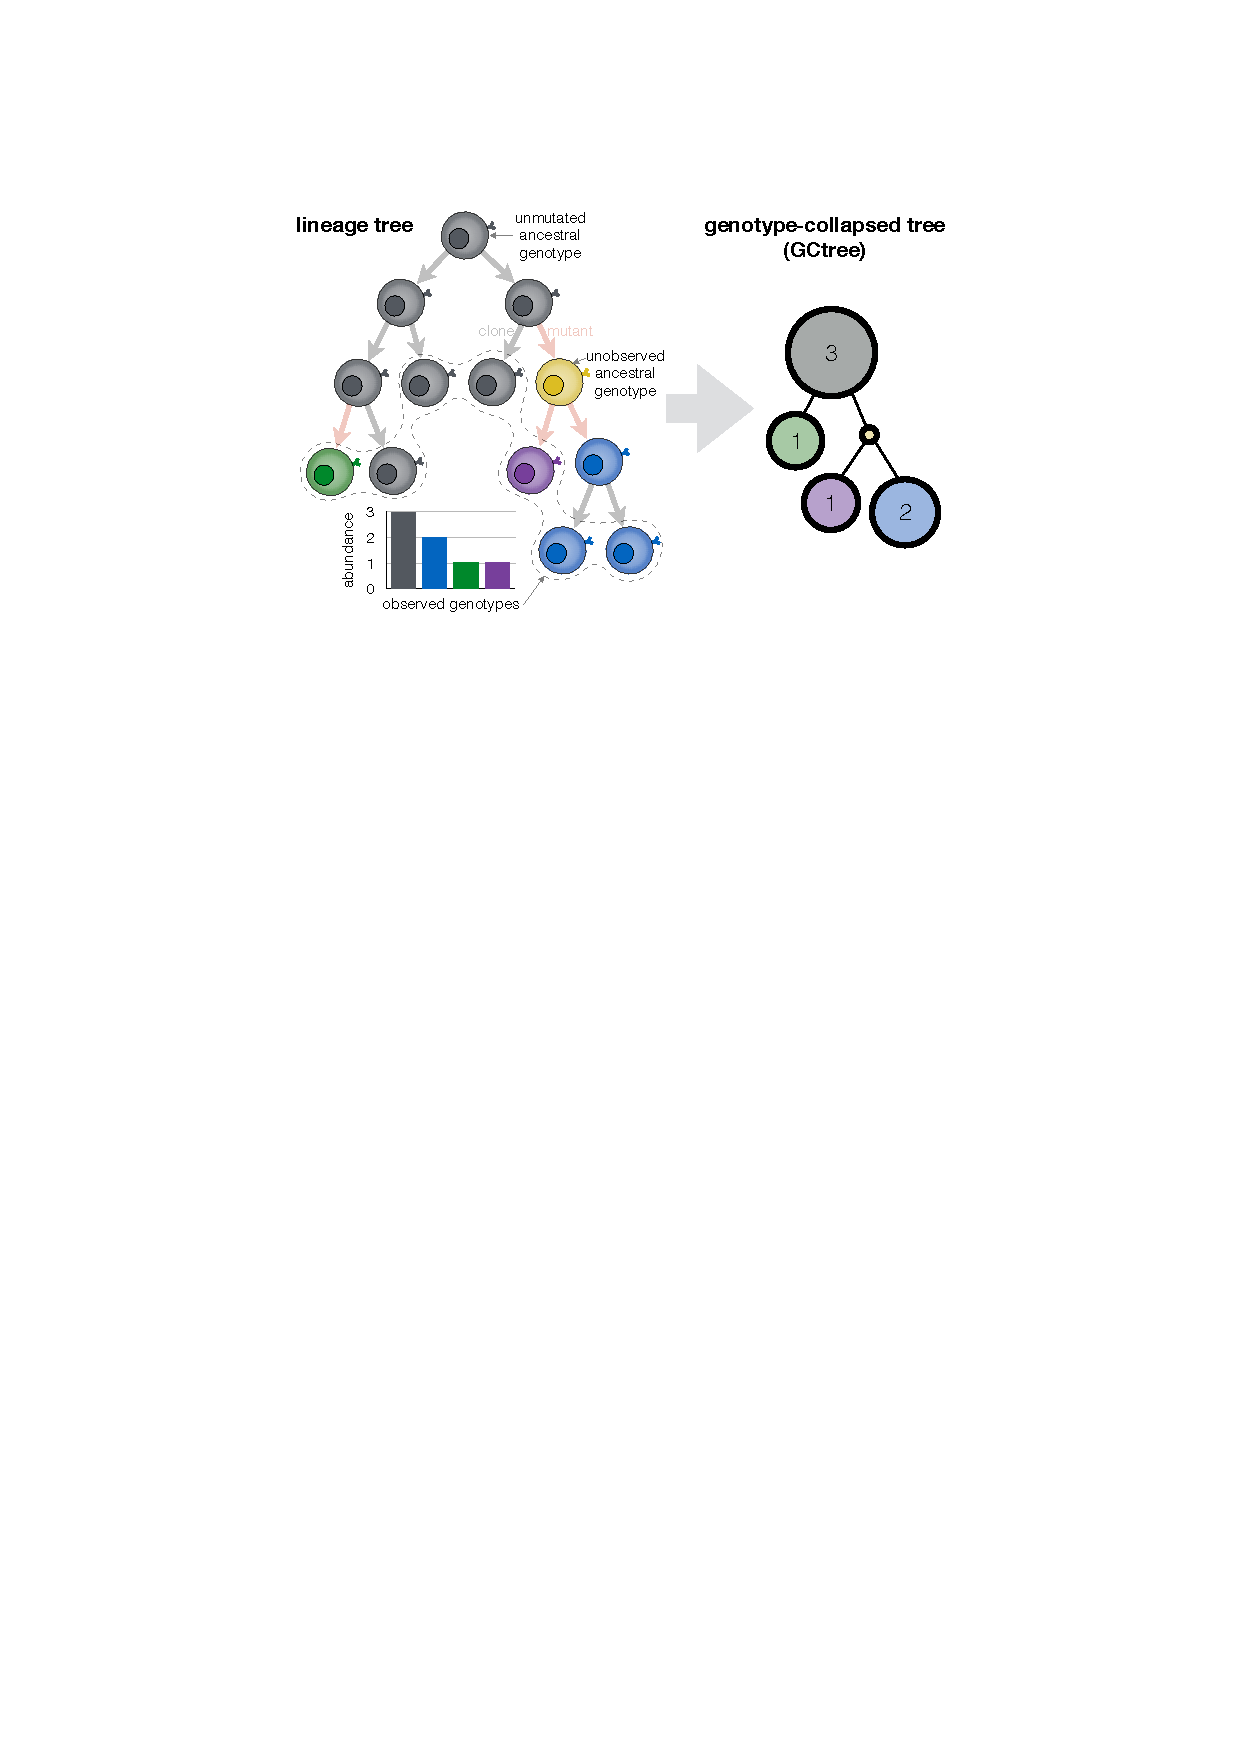
\includegraphics[width=0.7\textwidth]{figures/GCtree_illu.pdf}
    \caption{
        \label{fig:GCtree_illu}
        Genotype collapsed tree.
        Observed cells fenced by a dashed line are getting deduplicated and the total abundance is recorded.
        Next the tree is collapsed upwards, merging cells of the same genotype, ending up with the tree to the right.
        Figure credit: William S. DeWitt.
    }
\end{figure}


We find that the GCtree gives a good visual overview of the BCR phylogeny enabling interpretations such as recent clonal bursts, fitness advantages etc.
In the rest of this work all trees will be shown as a GCtree using custom tree plotting from the ETE package \cite{huerta2016ete}.
Figure \ref{fig:collapsed_tree_example} is an example of how a standard phylogenetic tree is collapsed and represented in GCtree format.
Embedded in the GCtree visualization is a number of traits: genotype abundance is annotated in the middle of each node and proportional to the node size, dashed branches represents synonymous mutations while fully drawn lines are non-synonymous, branch length is proportional to the hamming distance between nodes and branch thickness is proportional to the number of amino acid differences.

\begin{figure}[!ht]
    \centering
    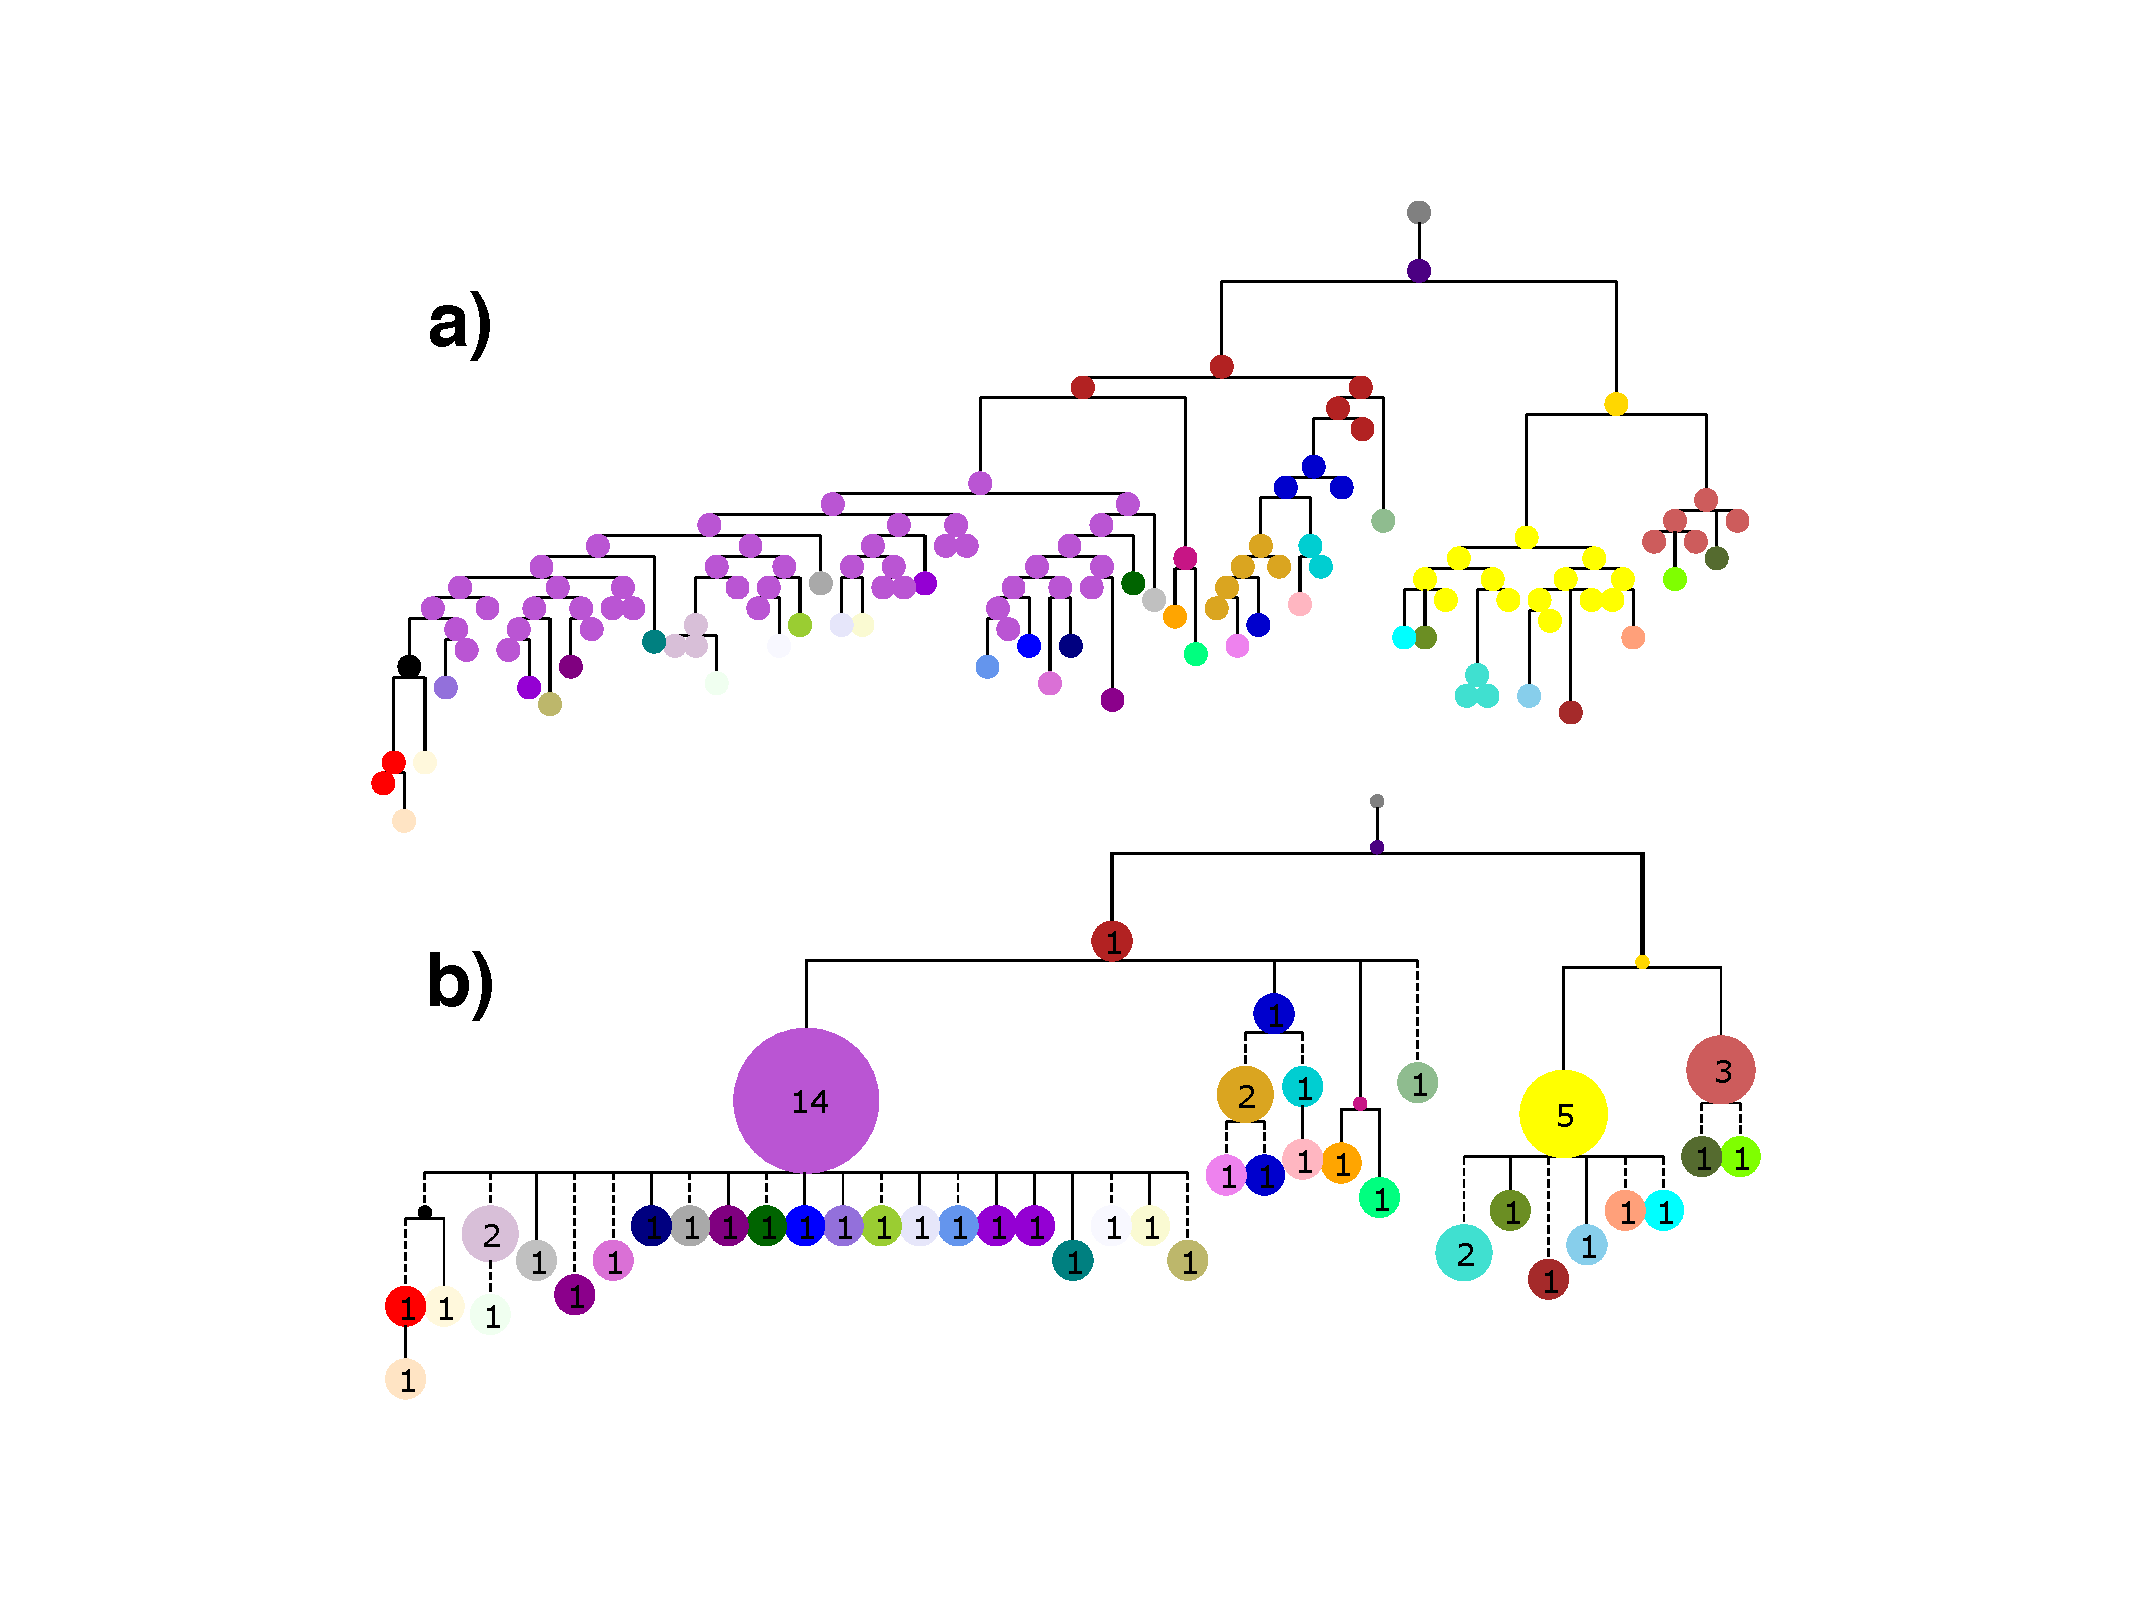
\includegraphics[width=0.7\textwidth]{figures/collapsed_tree_example.pdf}
    \caption{
        \label{fig:collapsed_tree_example}
        Genotype collapsing of a simulated tree with node coloring according to genotype.
        In a) a full lineage tree showing a simulation of several rounds of replication.
        Only the leafs are sampled at the end of the simulation and collapsed into the GCtree in b).
        The GCtree shows the leaf abundance of each node by way of node size and the integer in the middle of the node.
        In the GCtree synonymous mutations are indicated by dashed branch lines, branch length is reflecting the hamming distance between nodes at DNA level and solid branch line thickness reflects the number of non-synonymous mutations.
    }
\end{figure}





\subsection{Clonal family tree}
Most often the source of BCR sequences is HTS data generated from bulk RNA, extracted from peripheral blood mononuclear cells (PBMCs).
Clonal family relationships therefore needs to be inferred by means of clustering before sequences can be inputted to phylogenetic tools.
An automated pipeline can be envisioned, with HTS data as input and inferred clonal family trees as output.
One attempt at this task is the publicly available ImmuneDB \cite{rosenfeld2017immunedb}.
Using relatively simple clustering and inference of naive sequences ImmuneDB still has room for improvements, but the concept remains extremely important as a way of aiding the interpretation of Rep-Seq data.
On the conceptual side of the clonal family tree representation is it possible to map meta information about binding affinity, cross reactivity, self-binding etc. back to individual trees to get a detailed picture of the evolutionary process at a single cell level.






